\documentclass[aspectratio=169,12pt]{beamer}
\usepackage[utf8]{inputenc}
\usepackage{amsmath, amssymb}
\usepackage{booktabs}
\usepackage{colortbl}
\usepackage{hyperref}
\usepackage{listings}
\usepackage{makecell}
\usepackage{ragged2e}
\usepackage{bytefield}
\usepackage{tikz}
\usetikzlibrary{arrows.meta, positioning, shapes.geometric, calc, tikzmark}
\usetheme{Madrid}

% Define colors for registers
\definecolor{r1color}{RGB}{255,0,0}
\definecolor{r2color}{RGB}{0,128,0}
\definecolor{r3color}{RGB}{255,165,0}
\definecolor{r4color}{RGB}{128,0,128}
\definecolor{r5color}{RGB}{0,0,255}
\definecolor{r6color}{RGB}{255,165,0}
\definecolor{r7color}{RGB}{0,0,0}
\definecolor{r8color}{RGB}{0,128,0}

% Define hyphenation command
\newcommand{\hyp}{\-}

% Proportional widths for the table-only version
\newlength\TotalW
\setlength\TotalW{\textwidth}
\newlength\Wone    \setlength\Wone   {0.015625\TotalW} % 1/64
\newlength\Weleven \setlength\Weleven{0.171875\TotalW} % 11/64
\newlength\Wforty  \setlength\Wforty {0.625000\TotalW} % 40/64
\newlength\Wtwelve \setlength\Wtwelve{0.187500\TotalW} % 12/64
\newcolumntype{L}[1]{>{\RaggedRight\arraybackslash}p{#1}}
\newcolumntype{C}[1]{>{\Centering\arraybackslash}p{#1}}
\renewcommand{\arraystretch}{1.2}

% Show slide number as "current/total" in the footer
\setbeamertemplate{footline}{%
  \leavevmode\hbox{\begin{beamercolorbox}[wd=\paperwidth,ht=2.25ex,dp=1ex,center]{author in head/foot}%
    \usebeamerfont{author in head/foot}\insertframenumber/\inserttotalframenumber
  \end{beamercolorbox}}%
  \vskip0pt%
}
\setbeamertemplate{navigation symbols}{}
\title{Computer Structure\\Virtual Memory}
\author{Based on slides by Lihu Rappoport}
\date{}
\begin{document}

\frame{\titlepage}

\begin{frame}{Virtual Memory}
\begin{itemize}
\item \textbf{Provide isolation:} each process sees its own memory space
    \begin{itemize}
    \item Many processes can run on a single machine
    \item Prevents a process from accessing the memory of other processes
    \end{itemize}
\item \textbf{Provides the illusion of a large memory for each process}
    \begin{itemize}
    \item Different machines have different amount of physical memory
    \item Allows programs to run regardless of actual physical memory size
    \item Sum of memory spaces of all process may be larger than physical memory
    \end{itemize}
\item \textbf{Provides illusion of contiguous memory}
    \begin{itemize}
    \item The amount of memory consumed by each process is dynamic
    \item Allows adding memory and keep it contiguous
    \end{itemize}
\end{itemize}
\end{frame}

\begin{frame}{Virtual Address Spaces}
\begin{center}
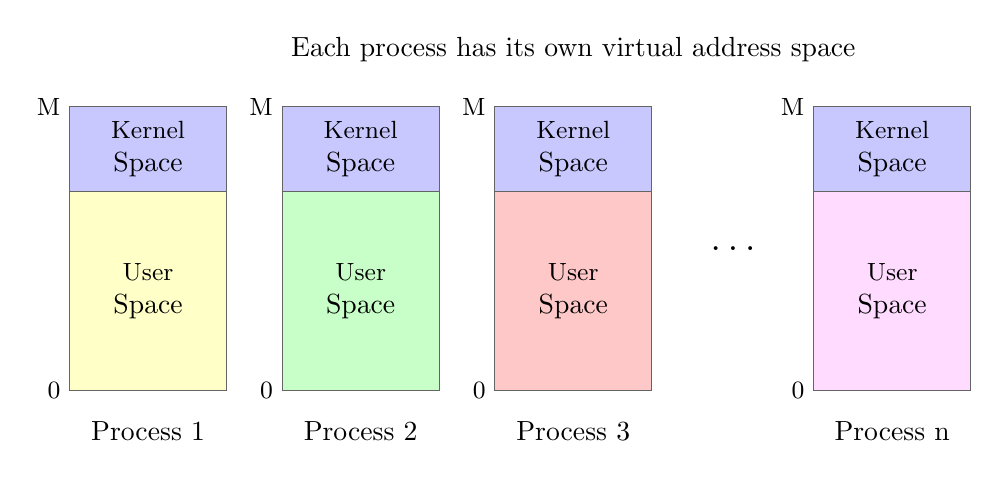
\begin{tikzpicture}[scale=0.9]
    % Define colors
    \definecolor{kernelcolor}{RGB}{200,200,255}
    \definecolor{usercolor1}{RGB}{255,255,200}
    \definecolor{usercolor2}{RGB}{200,255,200}
    \definecolor{usercolor3}{RGB}{255,200,200}
    \definecolor{usercolor4}{RGB}{255,220,255}
    \definecolor{bordercolor}{RGB}{100,100,100}
    
    % Define dimensions
    \def\procwidth{2.2}
    \def\procheight{4}
    \def\kernelheight{1.2}
    \def\spacing{0.8}
    \pgfmathsetmacro{\kernelcenter}{\procheight-\kernelheight/2}
    \pgfmathsetmacro{\usercenter}{(\procheight-\kernelheight)/2}
    
    % Draw processes using foreach loop
    \foreach \i in {0, 1, 2} {
        \begin{scope}[shift={({\i*(\procwidth+\spacing)},0)}]
            \draw[thick, bordercolor] (0,0) rectangle (\procwidth,\procheight);
            
            % Kernel space (top)
            \fill[kernelcolor] (0,\procheight-\kernelheight) rectangle (\procwidth,\procheight);
            \draw[thick, bordercolor] (0,\procheight-\kernelheight) -- (\procwidth,\procheight-\kernelheight);
            
            % User space (bottom) - different color for each process
            \pgfmathtruncatemacro{\colornum}{\i+1}
            \fill[usercolor\colornum] (0,0) rectangle (\procwidth,\procheight-\kernelheight);
            
            % Labels with two lines
            \node[align=center] at (\procwidth/2, \kernelcenter) {\small Kernel\\Space};
            \node[align=center] at (\procwidth/2, \usercenter) {\small User\\Space};
            
            % Address labels
            \node[left] at (0, \procheight) {\small M};
            \node[left] at (0, 0) {\small 0};
            
            % Process label
            \pgfmathtruncatemacro{\procnum}{\i+1}
            \node[below] at (\procwidth/2, -0.3) {Process \procnum};
        \end{scope}
    }
    
    % Dots indicating more processes
    \node at ({{3*(\procwidth+\spacing) + \spacing/2}}, \procheight/2) {\Large \ldots};
    
    % Process n
    \begin{scope}[shift={({3.5*(\procwidth+\spacing)},0)}]
        \draw[thick, bordercolor] (0,0) rectangle (\procwidth,\procheight);
        
        % Kernel space (top)
        \fill[kernelcolor] (0,\procheight-\kernelheight) rectangle (\procwidth,\procheight);
        \draw[thick, bordercolor] (0,\procheight-\kernelheight) -- (\procwidth,\procheight-\kernelheight);
        
        % User space (bottom) - use color 4 for process n
        \fill[usercolor4] (0,0) rectangle (\procwidth,\procheight-\kernelheight);
        
        % Labels with two lines
        \node[align=center] at (\procwidth/2, \kernelcenter) {\small Kernel\\Space};
        \node[align=center] at (\procwidth/2, \usercenter) {\small User\\Space};
        
        % Address labels
        \node[left] at (0, \procheight) {\small M};
        \node[left] at (0, 0) {\small 0};
        
        % Process label
        \node[below] at (\procwidth/2, -0.3) {Process n};
    \end{scope}
    
    % Title/description
    \node[above, font=\normalsize] at ({2.5*\procwidth + 2*\spacing}, \procheight + 0.5) {Each process has its own virtual address space};
    
\end{tikzpicture}
\end{center}
\end{frame}

\begin{frame}{Virtual Memory: Basic Idea}
\begin{itemize}
\item \textbf{Basic terminology}
    \begin{itemize}
    \item Virtual Address Space (per process): address space used by the process
    \item Physical Address: actual physical memory address space
    \end{itemize}
\item \textbf{Divide each space (virtual and physical) into fixed size blocks}
    \begin{itemize}
    \item Pages in Virtual space, Frames in Physical space
    \item Page size = Frame size = some power of 2
    \end{itemize}
\item \textbf{Virtual pages are mapped either to}
    \begin{itemize}
    \item A physical frame in memory
    \item Or a sector in the disk
    \end{itemize}
\item \textbf{All addresses in programs use Virtual Memory Address Space}
    \begin{itemize}
    \item Hardware translates virtual to physical addresses on-the-fly
    \item Uses a Page Table for the translation
    \end{itemize}
\end{itemize}
\end{frame}

\begin{frame}{Page Tables}
\begin{itemize}
\item The OS manages a page table for each process
    \begin{itemize}
    \item The OS maps the process virtual pages to physical pages or to disk
    \item Only the OS writes into the page tables
    \item The page tables reside in the physical memory (DRAM)
    \end{itemize}
\end{itemize}
\begin{center}
[Diagram: Page Table mapping Virtual Pages to Physical Pages and Disk with Present bits]
\end{center}
\end{frame}

\begin{frame}{Virtual to Physical Address Translation}
\begin{itemize}
\item PTE – Page Table Entry
\item Page size: $2^{12}$ byte = 4K byte
\end{itemize}
\begin{center}
[Diagram showing virtual address (47-12 bits VPN, 11-0 bits offset) mapping to physical address]
\end{center}
Components:
\begin{itemize}
\item Page table base reg
\item Present bit, Dirty bit
\item Access Control (Memory type, User/Supervisor)
\item Physical page number
\end{itemize}
\end{frame}

\begin{frame}{Page Table Location}
\begin{itemize}
\item The page table of each process resides in main memory
    \begin{itemize}
    \item When a process is running, the start address of its page table is pointed by a special register in the CPU: the page table base register
    \item The page table base register holds the physical address of entry 0
    \end{itemize}
\item The physical address of the PTE of virtual page \#VPN
    \begin{itemize}
    \item PTE address = Page table base reg + VPN $\times$ PTE\_size
    \end{itemize}
\end{itemize}
\end{frame}

\begin{frame}{Mapping Virtual Address Spaces to Physical Memory}
\begin{itemize}
\item Each process has its own address space $\rightarrow$ each process has its own page table
    \begin{itemize}
    \item A process cannot access physical memory allocated to another process (unless OS intentionally shares some of it)
    \end{itemize}
\item On a context switch, the Page Table Base Register is loaded with the page table base address of the process that moves in
\end{itemize}
\begin{center}
[Diagram: Multiple process virtual address spaces mapping to physical memory]
\end{center}
\end{frame}

\begin{frame}{Page Fault and Protection Violation Fault}
\textbf{If present bit in the page table entry == 0 then // page fault}
\begin{itemize}
\item Page is not mapped to main memory $\rightarrow$ need to retrieve it from disk
\item The CPU detects the situation, but cannot remedy it $\rightarrow$ traps to the OS
\item The OS takes care of the page fault:
    \begin{itemize}
    \item If there is no free space in physical memory:
        \begin{itemize}
        \item Picks a physical page to discard (based on some replacement policy)
        \item Marks the page as not present in the page table
        \item Copies the page to the disk swap area
        \end{itemize}
    \item Loads the new page from disk into the selected physical page
    \item Updates the page table entry of the new page
    \item Resumes to the program so HW retries and succeeds
    \end{itemize}
\end{itemize}
\textbf{When a page is present the CPU checks the page access control bits}
\begin{itemize}
\item R = Read-only, R/W = read/write, X = execute only
\item If access type is not compatible with the specified access rights $\rightarrow$ protection violation fault
\end{itemize}
\end{frame}

\begin{frame}{Optimal Page Size}
\begin{itemize}
\item \textbf{Minimize wasted storage}
    \begin{itemize}
    \item Small pages minimize internal fragmentation
    \item Small pages increase the size of the page tables
    \end{itemize}
\item \textbf{Minimize transfer time – use large pages (multiple disk sectors)}
    \begin{itemize}
    \item Amortize access cost and prefetch useful data
    \item But, might transfer unnecessary data and discard (victimize) useful data
    \end{itemize}
\item \textbf{General trend toward larger pages because}
    \begin{itemize}
    \item Big cheap RAM
    \item Increasing memory / disk performance gap
    \item Larger address spaces
    \item Programs with larger code and data
    \end{itemize}
\end{itemize}
\end{frame}

\begin{frame}{Translation Look aside Buffer (TLB)}
\begin{itemize}
\item With virtual memory, before each cache access, need to first get the physical address
    \begin{itemize}
    \item The page table resides in memory $\rightarrow$ each translation requires an extra memory access
    \end{itemize}
\item The TLB is a cache for recent address translations
\end{itemize}
\begin{center}
[Diagram: TLB caching page table entries]
\end{center}
\end{frame}


\begin{frame}{Translation Look aside Buffer (TLB)}
\begin{columns}[T]
\begin{column}{0.57\textwidth}
\begin{itemize}
\item \textbf{The TLB caches recently used PTEs}
\item[] Typically, 128--256 entries, 4--8 ways
    
\item \textbf{TLB Indexing}

\begin{center}
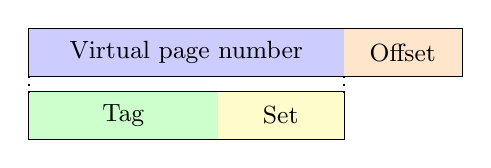
\begin{tikzpicture}[scale=1]
    % Virtual address breakdown
    \draw[thick] (0,0) rectangle (5.5,0.6);
    \draw[thick] (4,0) -- (4,0.6);
    
    % Fill colors
    \fill[blue!20] (0,0) rectangle (4,0.6);
    \fill[orange!20] (4,0) rectangle (5.5,0.6);
    
    % Labels
    \node at (2,0.3) {\small Virtual page number};
    \node at (4.75,0.3) {\small Offset};
    
    % Tag and Set subdivision
    \draw[thick] (0,-0.8) rectangle (4,-0.2);
    \draw[thick] (2.4,-0.8) -- (2.4,-0.2);
    
    \fill[green!20] (0,-0.8) rectangle (2.4,-0.2);
    \fill[yellow!20] (2.4,-0.8) rectangle (4,-0.2);
    
    \node at (1.2,-0.5) {\small Tag};
    \node at (3.2,-0.5) {\small Set};
    
    % Dotted lines connecting
    \draw[dotted, thick] (0,0) -- (0,-0.2);
    \draw[dotted, thick] (4,0) -- (4,-0.2);
\end{tikzpicture}
\end{center}

\item \textbf{On A TLB miss}
    \begin{itemize}
    \item Page Miss Handler (PMH) loads address PTBR+VPN$\times$PTE\_size to read PTE
    \item PMH may contain a 2\textsuperscript{nd} level TLB
    \end{itemize}
    
\item \textbf{OS maintains TLB coherency}
\item[] OS updates PTE $\rightarrow$ OS must invalidate PTE in TLB
\end{itemize}
\end{column}

\begin{column}{0.43\textwidth}
\begin{center}
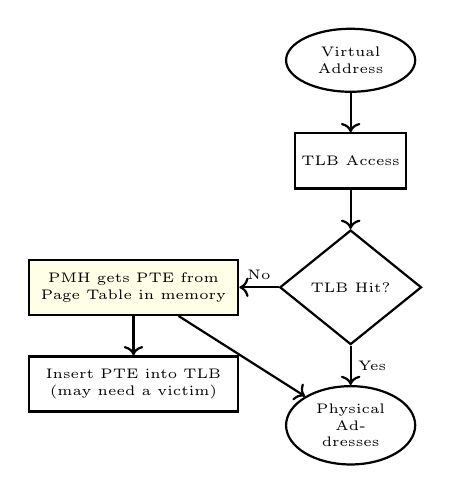
\begin{tikzpicture}[
    node distance=5mm,
    box/.style={rectangle, draw, thick, minimum width=1cm, minimum height=0.7cm, text centered, font=\tiny},
    decision/.style={diamond, draw, thick, minimum width=1.8cm, minimum height=1cm, text centered, font=\tiny},
    oval/.style={ellipse, draw, thick, minimum width=1cm, minimum height=0.8cm, text centered, font=\tiny, text width=1cm},
    arrow/.style={->, thick}]
    \tiny
    % Nodes
    \node[oval, align=center] (va) {Virtual Address};
    \node[box, align=center, below=of va] (tlb) {TLB Access};
    \node[decision, below=of tlb] (hit) {TLB Hit?};
    \node[box, fill=yellow!10, align=center, left=of hit, text width=2.5cm] (pmh) {PMH gets PTE from Page Table in memory};
    \node[box, align=center, below=of pmh, text width=2.5cm] (insert) {Insert PTE into TLB (may need a victim)};
    \node[oval, align=center, below=of hit] (pa) {Physical Addresses};
    
    % Arrows
    \draw[arrow] (va) -- (tlb);
    \draw[arrow] (tlb) -- (hit);
    \draw[arrow] (hit) -- node[above] {No} (pmh);
    \draw[arrow] (hit) -- node[right] {Yes} (pa);
    \draw[arrow] (pmh) -- (insert);
    \draw[arrow] (pmh) -- (pa);
    
\end{tikzpicture}
\end{center}
\end{column}
\end{columns}
\end{frame}

\begin{frame}{Processor Caches and TLBs}
\begin{itemize}
\item Each of L1 I\$ and L1 D\$ has its own TLB – ITLB and DTLB
    \begin{itemize}
    \item Similar to the I\$ and the D\$, the ITLB and DTLB are accessed in different pipe-stages
    \end{itemize}
\item In case of either ITLB or DTLB miss: access the STLB (second level TLB)
\item In case of STLB miss
    \begin{itemize}
    \item PMH (page miss handler) injects a load to get the PTE from the page table (page walk)
    \item This load, like any other load, starts by a lookup in the L1 D\$
    \end{itemize}
\end{itemize}
\begin{center}
[Diagram: Core with L1 I\$, L1 D\$, ITLB, DTLB, STLB, L2, L3, and Memory hierarchy]
\end{center}
\end{frame}

\begin{frame}{Virtual Memory and Cache}
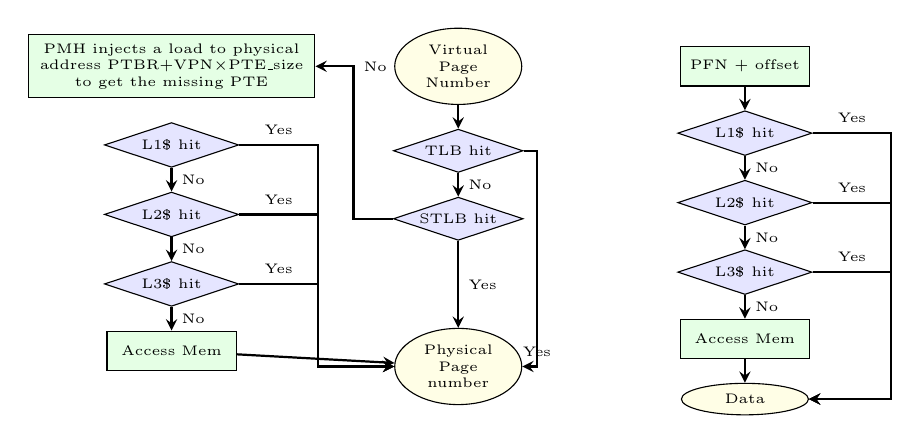
\begin{tikzpicture}[
    node distance=3mm,
    decision/.style={diamond, draw, fill=blue!10, text width=1cm, align=center, inner sep=1pt, minimum height=0.3cm, aspect=3, font=\tiny},
    process/.style={rectangle, draw, fill=green!10, text width=1.5cm, align=center, minimum height=0.5cm, inner sep=2pt, font=\tiny},
    data/.style={ellipse, draw, fill=yellow!10, text width=1cm, align=center, minimum height=0.4cm, inner sep=2pt, font=\tiny},
    arrow/.style={->, >=stealth, thick},
    every node/.style={font=\tiny}
]

% Top section - TLB lookup
\node[data] (vpn) {Virtual Page Number};
\node[decision, below=of vpn] (tlb) {TLB hit};
\node[decision, below=of tlb] (stlb) {STLB hit};

% Translation path
\node[process, left=1cm of vpn, text width=3.5cm, minimum height=0.8cm] (pmh) {PMH injects a load to physical address PTBR+VPN$\times$PTE\_size to get the missing PTE};
%\node[process, below=of pmh] (trans) {Get the Translation};
\node[decision, below=of pmh] (l1) {L1\$ hit};
\node[decision, below=of l1] (l2) {L2\$ hit};
\node[decision, below=of l2] (l3) {L3\$ hit};
\node[process, below=of l3] (mem1) {Access Mem};

\node[data] (pfn) at ([yshift=-2mm]mem1 -| stlb) {Physical Page number};


% Data path
\node[process, right=2cm of vpn] (getdata) {PFN + offset};
\node[decision, below=of getdata] (l1d) {L1\$ hit};
\node[decision, below=of l1d] (l2d) {L2\$ hit};
\node[decision, below=of l2d] (l3d) {L3\$ hit};
\node[process, below=of l3d] (mem2) {Access Mem};
\node[data, below=of mem2] (data) {Data};

% Arrows
\draw[arrow] (vpn) -- (tlb);
\draw[arrow] (tlb) -- node[right] {No} (stlb);
\draw[arrow] (tlb) -- ++(1,0) |- node[above] {Yes} (pfn);
\draw[arrow] (stlb.west) -- ++(-0.5, 0) |- node[right] {No} (pmh.east);
\draw[arrow] (stlb.south) -- node[right] {Yes} (pfn);
%\draw[arrow] (pmh) -- (l1);
\draw[arrow] (l1) -- node[right] {No} (l2);
\draw[arrow] (l2) -- node[right] {No} (l3);
\draw[arrow] (l3) -- node[right] {No} (mem1);
\draw[arrow] (l1.east) -- node[above] {Yes} ++(1,0) |- (pfn);
\draw[arrow] (l2.east) -- node[above] {Yes} ++(1,0) |- (pfn);
\draw[arrow] (l3.east) -- node[above] {Yes} ++(1,0) |- (pfn);
\draw[arrow] (mem1) -- (pfn);
%\draw[arrow] (pmh) |- (getdata);
%\draw[arrow] (pfn) |- node[near end, above] {PFN offset} (getdata);
\draw[arrow] (getdata) -- (l1d);
\draw[arrow] (l1d) -- node[right] {No} (l2d);
\draw[arrow] (l2d) -- node[right] {No} (l3d);
\draw[arrow] (l3d) -- node[right] {No} (mem2);
\draw[arrow] (l1d.east) -- node[above] {Yes} ++(1,0) |- (data);
\draw[arrow] (l2d.east) -- node[above] {Yes} ++(1,0) |- (data);
\draw[arrow] (l3d.east) -- node[above] {Yes} ++(1,0) |- (data);
\draw[arrow] (mem2.south) -- (data);

\end{tikzpicture}

\footnotesize
\begin{itemize}
\item Page table entries are cached in L1 D\$, L2\$ and L3\$ as data
\item If the injected load misses in a cache $\Rightarrow$ perform a cache line fill $\Rightarrow$ all PTEs in the missed cached line are brought into the cache
\item Only the specific missed PTE is filled into the STLB and TLB
\end{itemize}
\end{frame}


\begin{frame}{Virtual Memory And Cache}
\begin{itemize}
\item Page table entries are cached in L1 D\$, L2\$ and L3\$ as data
\item If the injected load misses in a cache $\rightarrow$ perform a cache line fill
    \begin{itemize}
    \item all PTEs in the missed cached line are brought into the cache
    \end{itemize}
\item Only the specific missed PTE is filled into the STLB and TLB
\end{itemize}
\textbf{Get the Translation:}
Virtual Page Number $\rightarrow$ TLB hit? $\rightarrow$ STLB hit? $\rightarrow$ PMH $\rightarrow$ L1\$/L2\$/L3\$/Mem

\textbf{Get the Data:}
PFN + offset $\rightarrow$ L1\$ hit? $\rightarrow$ L2\$ hit? $\rightarrow$ L3\$ hit? $\rightarrow$ Access Mem
\end{frame}

\begin{frame}{Overlapping TLB \& Cache Access}
\textbf{Goal:} start cache access in parallel to TLB access
\begin{itemize}
\item Save a cycle on getting the data in case of TLB hit and cache hit
\end{itemize}

\textbf{Cache \#set contained in page offset}
\begin{itemize}
\item Cache set available before translation
\item Access cache set in parallel with TLB
\item Once translation is done, match physical page number with tag of each way
\end{itemize}

\textbf{Restriction on cache}
\begin{itemize}
\item \#sets $\times$ line size = way size $\leq$ page size
\item Cache size $\leq$ page size $\times$ associativity
\end{itemize}
\end{frame}

\begin{frame}{Evicting a Page to Disk}
\textbf{OS updates the Page Table}
\begin{itemize}
\item OS invalidate the page from the TLBs (using a special instruction)
    \begin{itemize}
    \item It is the OS responsibility to maintain coherency between page table and TLBs for any change in the page table
    \end{itemize}
\item OS marks the swapped-out page as not present (present=0) in its PTE
    \begin{itemize}
    \item If the PTE is cached in any of the caches, MESI protocol maintains coherency
    \end{itemize}
\item OS writes the page disk location into the PTE
\end{itemize}

\textbf{OS copies the page to the disk}
\begin{itemize}
\item Read each block (=cache line) within the page
\item Snoop-invalidate each line in the CPUs caches
\item Write the block to the disk-controller Memory-Mapped I/O area
\end{itemize}
\end{frame}

\begin{frame}{Context Switch}
\textbf{On a context switch}
\begin{itemize}
\item Save the current architectural state to a dedicated memory location
    \begin{itemize}
    \item HW supports fast save command
    \item Architectural registers, including the page-table base-address register
    \end{itemize}
\item Flush the TLBs
\item Load the new architectural state from memory
    \begin{itemize}
    \item Architectural registers, including the page-table base-address register
    \end{itemize}
\end{itemize}
\end{frame}


\begin{frame}{Virtually-Addressed Cache}
\begin{itemize}
\item \textbf{Cache uses virtual addresses (tags are virtual)}
\item \textbf{Address translation only done on a cache miss}
    \begin{itemize}
    \item TLB is not in the path to cache hit
    \end{itemize}
\end{itemize}

\vspace{-0.1cm}
\begin{center}
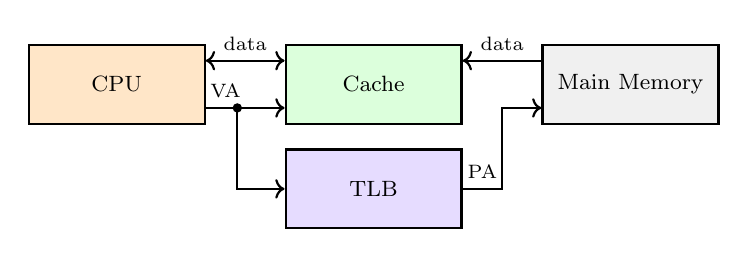
\begin{tikzpicture}[
    box/.style={rectangle, draw, thick, minimum width=1.8cm, minimum height=1cm, text centered, text width=2cm, font=\footnotesize},
    data_connector/.style={circle, fill, inner sep=1.2pt},
    arrow/.style={->, thick, font=\scriptsize, yshift=-2mm},
    doublearrow/.style={<->, thick, font=\scriptsize, yshift=-2mm}]
    
    % Define colors
    \definecolor{cpucolor}{RGB}{255,230,200}
    \definecolor{cachecolor}{RGB}{220,255,220}
    \definecolor{tlbcolor}{RGB}{230,220,255}
    \definecolor{memcolor}{RGB}{240,240,240}
    
    % Nodes
    \node[box, fill=cpucolor] (cpu) {CPU};
    \node[box, fill=cachecolor, right=of cpu] (cache) {Cache};
    \node[box, fill=memcolor, align=center, right=of cache] (memory) {Main Memory};
    \node[box, fill=tlbcolor, below=3mm of cache] (tlb) {TLB};
    
    % Arrows with labels
    % CPU to Cache - bidirectional with VA going right, data going left
    %\draw[arrow] (cpu.east) -- node[above] {\small VA} (cache.west);
    %\draw[arrow] (cache.west) -- +(-0.7,0) -- +(-0.7,0.3) -- ($(cpu.east) + (0,0.3)$) -- node[above, pos=0.7] {\small data} (cpu.east |- {$(cpu.east) + (0,0.3)$});
    
    \draw[doublearrow] ([yshift=3mm]cache.west) -- node[above] {data} ([yshift=3mm]cpu.east);
    
    \draw[arrow] ([yshift=-3mm]cpu.east) -- node[above, near start] {VA} ([yshift=-3mm]cache.west);
    
    % TLB to Memory - PA
    \draw[arrow] (tlb.east) -- node[above] {PA} ++(0.5,0) |- ([yshift=-3mm]memory.west);
    \draw[arrow] ([yshift=3mm]memory.west) -- node[above] {data} ([yshift=3mm]cache.east);
    \draw[arrow] ([xshift=4mm, yshift=-3mm]cpu.east) node[data_connector] {} |- (tlb.west);
    
\end{tikzpicture}
\end{center}

\vspace{0.1cm}
\begin{itemize}
\item \textbf{Two virtual pages mapped to the same physical page}
    \begin{itemize}
    \item Must not reside in the cache together
    \item On a cache miss, use a reverse TLB to verify that no other cache line already in the cache mapped to the missed physical address
    \end{itemize}
    
\item \textbf{Flush cache on context switch}
    \begin{itemize}
    \item Alternatively: add process ID as part of the tag
    \end{itemize}
\end{itemize}
\end{frame}

\begin{frame}{Paging in x86}
\begin{center}
\Huge Paging in x86
\end{center}
\end{frame}

\begin{frame}{Page Tables Size}
\textbf{Assume}
\begin{itemize}
\item A virtual address space of size $2^{48}$ bytes
\item A page size of 4KB = $2^{12}\text{B} \rightarrow \frac{2^{48}\text{B}}{2^{12}\text{B}} = 2^{36}$ entries in the page table
\item A PTE size of 8 bytes $\rightarrow$ page table size is $2^{36} \times 8$B = $2^{39}$B
\item 128 process running in the system, each with it own page table $\rightarrow$ $2^{39}$B $\times$ 128 = $2^{46}$B
\item Page tables alone requires a huge physical memory
\end{itemize}

\textbf{Solution}
\begin{itemize}
\item Most processes use a small portion of the virtual address space
\item Use hierarchical page tables – the page table of each process maps the pages that the process is actually using (allocated to), and not the entire virtual address space
\item The hierarchical page table is split into pages
\item Some of the pages in the page table hierarchy may be not in physical memory
    \begin{itemize}
    \item In case getting to such a page, the CPU traps to the OS to get the page
    \end{itemize}
\end{itemize}
\end{frame}


\begin{frame}{4KB Page Mapping in 64-bit Mode}
\begin{columns}[T]
\begin{column}{0.44\textwidth}
\begin{itemize}
\item \textbf{4-level hierarchical paging}
\item Each page table: 4KB in size
\item Each page table entry (PTE): 8B
\item Entries per table: $\frac{4\text{KB}}{8\text{B}} = 512 = 2^9$
\item Level $n$ entry points to level $n-1$ table base
    \begin{itemize}
    \item[$\triangleright$] Provides $(M-12)$ address bits
    \item[$\triangleright$] Bits [11:0] = 0 (4KB-aligned)
    \item[$\triangleright$] $M = \log_2(\text{physical mem size})$
    \item[$\triangleright$] CR3 register $\rightarrow$ PML4 base
    \end{itemize}
\item 9 VA bits $\rightarrow$ index in each table
\item VA[11:0] byte offset in 4KB page
\end{itemize}
\end{column}

\begin{column}{0.56\textwidth}
\begin{center}
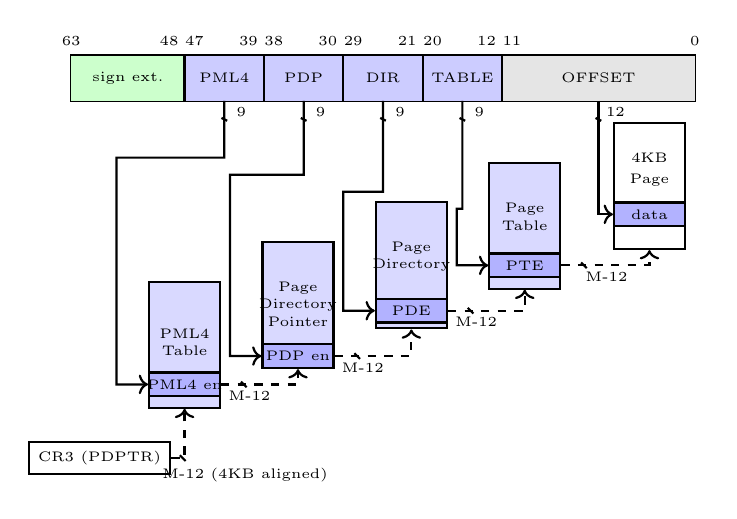
\begin{tikzpicture}[scale=0.72,
    table/.style={rectangle, draw, thick, minimum width=0.9cm, fill=blue!15},
    entry/.style={rectangle, draw, thick, minimum width=0.9cm, minimum height=0.3cm, fill=blue!30},
    data/.style={rectangle, draw, thick, minimum width=0.9cm, minimum height=1.6cm, fill=white},
    arrow/.style={->, thick},
    dashedarrow/.style={->, thick, dashed}]
    
    % Virtual Address breakdown at the top
    \draw[thick] (0,7.5) rectangle (11,8.3);
    
    % Address fields with colors
    \fill[green!20] (0,7.5) rectangle (2,8.3);
    \fill[blue!20] (2,7.5) rectangle (3.4,8.3);
    \fill[blue!20] (3.4,7.5) rectangle (4.8,8.3);
    \fill[blue!20] (4.8,7.5) rectangle (6.2,8.3);
    \fill[blue!20] (6.2,7.5) rectangle (7.6,8.3);
    \fill[gray!20] (7.6,7.5) rectangle (11,8.3);
    
    % Field separators
    \draw[thick] (2,7.5) -- (2,8.3);
    \draw[thick] (3.4,7.5) -- (3.4,8.3);
    \draw[thick] (4.8,7.5) -- (4.8,8.3);
    \draw[thick] (6.2,7.5) -- (6.2,8.3);
    \draw[thick] (7.6,7.5) -- (7.6,8.3);
    
    % Field labels above
    \node[above, font=\tiny] at (0,8.3) {63};
    \node[above, font=\tiny] at (1.95,8.3) {48 47};
    \node[above, font=\tiny] at (3.35,8.3) {39 38};
    \node[above, font=\tiny] at (4.75,8.3) {30 29};
    \node[above, font=\tiny] at (6.15,8.3) {21 20};
    \node[above, font=\tiny] at (7.55,8.3) {12 11};
    \node[above, font=\tiny] at (11,8.3) {0};
    
    \node[font=\tiny] at (1,7.9) {sign ext.};
    \node[font=\tiny] at (2.7,7.9) {PML4};
    \node[font=\tiny] at (4.1,7.9) {PDP};
    \node[font=\tiny] at (5.5,7.9) {DIR};
    \node[font=\tiny] at (6.9,7.9) {TABLE};
    \node[font=\tiny] at (9.3,7.9) {OFFSET};
    
    % Page table hierarchy - ascending from left to right with bigger vertical gaps
    % PML4 Table (lowest)
    \node[table, minimum height=1.6cm] (pml4) at (2,3.2) {};
    \node[font=\tiny] at (2,3.4) {PML4};
    \node[font=\tiny] at (2,3.1) {Table};
    \node[entry] (pml4en) at (2,2.5) {};
    \node[font=\tiny] at (pml4en) {PML4 en};
    
    % PDP Table (higher)
    \node[table, minimum height=1.6cm] (pdp) at (4,3.9) {};
    \node[font=\tiny] at (4,4.2) {Page};
    \node[font=\tiny] at (4,3.9) {Directory};
    \node[font=\tiny] at (4,3.6) {Pointer};
    \node[entry] (pdpen) at (4,3.0) {};
    \node[font=\tiny] at (pdpen) {PDP en};
    
    % Page Directory (higher)
    \node[table, minimum height=1.6cm] (dir) at (6,4.6) {};
    \node[font=\tiny] at (6,4.9) {Page};
    \node[font=\tiny] at (6,4.6) {Directory};
    \node[entry] (pde) at (6,3.8) {};
    \node[font=\tiny] at (pde) {PDE};
    
    % Page Table (even higher)
    \node[table, minimum height=1.6cm] (pt) at (8,5.3) {};
    \node[font=\tiny] at (8,5.6) {Page};
    \node[font=\tiny] at (8,5.3) {Table};
    \node[entry] (pte) at (8,4.6) {};
    \node[font=\tiny] at (pte) {PTE};
    
    % Data Page (highest) with data rectangle full width
    \node[data, minimum height=1.6cm] (datapage) at (10.2,6) {};
    \node[font=\tiny] at (10.2,6.5) {4KB};
    \node[font=\tiny] at (10.2,6.1) {Page};
    % Draw rectangle around "data" - full width of the page
    \node[entry] (databox) at (10.2,5.5) {};
    \node[font=\tiny] at (databox) {data};
    
    % CR3
    \node[rectangle, draw, thick, minimum width=1.2cm, minimum height=0.4cm] (cr3) at (0.5,1.2) {\tiny CR3 (PDPTR)};
    
    % Arrows from address fields to table entries (to west side) with "/" on line
    % PML4 arrow with "9" near origin and "/" on line
    \draw[arrow] (2.7,7.5) -- (2.7,6.5) -- (0.8,6.5) -- (0.8,2.5) -- (pml4en.west);
    \node[font=\tiny] at (3,7.3) {9};
    \draw[thick] (2.65,7.2) -- (2.75,7.15);
    
    % PDP arrow with "9" near origin and "/" on line
    \draw[arrow] (4.1,7.5) -- (4.1,6.2) -- (2.8,6.2) -- (2.8,3.0) -- (pdpen.west);
    \node[font=\tiny] at (4.4,7.3) {9};
    \draw[thick] (4.05,7.2) -- (4.15,7.15);
    
    % DIR arrow with "9" near origin and "/" on line
    \draw[arrow] (5.5,7.5) -- (5.5,5.9) -- (4.8,5.9) -- (4.8,3.8) -- (pde.west);
    \node[font=\tiny] at (5.8,7.3) {9};
    \draw[thick] (5.45,7.2) -- (5.55,7.15);
    
    % TABLE arrow with "9" near origin and "/" on line
    \draw[arrow] (6.9,7.5) -- (6.9,5.6) -- (6.8,5.6) -- (6.8,4.6) -- (pte.west);
    \node[font=\tiny] at (7.2,7.3) {9};
    \draw[thick] (6.85,7.2) -- (6.95,7.15);
    
    % OFFSET arrow to data box with "12" near origin and "/" on line
    \draw[arrow] (9.3,7.5) |- (databox.west);
    \node[font=\tiny] at (9.6,7.3) {12};
    \draw[thick] (9.25,7.2) -- (9.35,7.15);
    
    % Arrows connecting the hierarchy with bus width notation
    % CR3 to PML4 Table south (not PML4 en) - dashed
    \draw[dashedarrow] (cr3.east) -| (pml4.south);
    \draw[thick] ($(cr3.east) + (0.15,0.05)$) -- ($(cr3.east) + (0.25,-0.05)$);
    \node[font=\tiny] at ($(cr3.east) + (1.3,-0.3)$) {M-12 (4KB aligned)};
    
    % PML4 en to PDP Table south - dashed with "\" mark
    \draw[dashedarrow] (pml4en.east) -| (pdp.south);
    \draw[thick] ($(pml4en.east) + (0.35,0.05)$) -- ($(pml4en.east) + (0.45,-0.05)$);
    \node[font=\tiny] at ($(pml4en.east) + (0.5,-0.2)$) {M-12};
    
    % PDP en to Page Directory south - dashed with "\" mark
    \draw[dashedarrow] (pdpen.east) -| (dir.south);
    \draw[thick] ($(pdpen.east) + (0.35,0.05)$) -- ($(pdpen.east) + (0.45,-0.05)$);
    \node[font=\tiny] at ($(pdpen.east) + (0.5,-0.2)$) {M-12};
    
    % PDE to Page Table south - dashed with "\" mark
    \draw[dashedarrow] (pde.east) -| (pt.south);
    \draw[thick] ($(pde.east) + (0.35,0.05)$) -- ($(pde.east) + (0.45,-0.05)$);
    \node[font=\tiny] at ($(pde.east) + (0.5,-0.2)$) {M-12};
    
    % PTE to 4KByte Page (datapage) bottom - dashed with "\" mark
    \draw[dashedarrow] (pte.east) -| (datapage.south);
    \draw[thick] ($(pte.east) + (0.35,0.05)$) -- ($(pte.east) + (0.45,-0.05)$);
    \node[font=\tiny] at ($(pte.east) + (0.8,-0.2)$) {M-12};
    
\end{tikzpicture}
\end{center}
\end{column}
\end{columns}
\end{frame}



\begin{frame}{TLBs}
\textbf{The most recently used PDEs and PTEs are cached in TLBs}
\begin{itemize}
\item Separate TLB for data and instruction caches
\item Separate TLBs for 4KB, 2/4MB and 1GB page sizes
\item 2nd level TLB serves both instruction TLB and data TLB
\item TLB sizes in 6th Generation Intel® Core™ Processors:
\end{itemize}

\begin{center}
\footnotesize
\begin{tabular}{|l|c|c|c|}
\hline
 & \textbf{4KB pages} & \textbf{2MB/4MB Pages} & \textbf{1GB Pages} \\
\hline
Instruction TLBs & 128 entries, 8 ways & 8 entries / thread & none \\
\hline
Data TLBs & 64 entries, 4 ways & 32 entries, 4 ways & 4 entries, 4 ways \\
\hline
2nd level TLB & \multicolumn{2}{c|}{1536 entries, 12 ways (Shared by 4KB and 2/4MB pages)} & 16 entries, 4 ways \\
\hline
\end{tabular}
\end{center}

\textbf{In case of a hit in multiple TLBs}
\begin{itemize}
\item The largest page that hits is used
\end{itemize}
\end{frame}

\begin{frame}{PMH – Page Miss Handler}
\textbf{In case of an iTLB or a dTLB miss $\rightarrow$ Request PTE from PMH}
\begin{itemize}
\item PMH first tries the STLB (2nd level TLB) – save walk in case of an STLB hit
\item If STLB miss, PMH performs a page-walk: traverses the page table tree, starting at the root
\end{itemize}

\textbf{The PMH includes caches to shorten the page walk time}
\begin{itemize}
\item All 3 caches are accessed in parallel – use hit from the lowest table that hits
\item For each table that needs memory access PMH injects a "load"
\end{itemize}

\begin{center}
\footnotesize
\begin{tabular}{|l|l|l|l|}
\hline
\thead{cache} & \thead{Accessed with \\ VA bits} & \thead{If hits, \\ returns} & \thead{Saves accesses \\ to tables} \\
\hline
PDE cache & [47:21] & PDE & PTE \\
\hline
PDP cache & [47:30] & PDP entry & PDE and PTE \\
\hline
PML4 cache & [47:39] & PML4 entry & PDP, PDE, and PTE \\
\hline
\end{tabular}
\end{center}

\textbf{Page attributes}
\begin{itemize}
\item R/W flag: logical AND of R/W flag in all levels
\item U/S flag: logical OR of U/S flag in all levels
\item XD flag: logical OR of XD flag in all levels
\end{itemize}
\end{frame}

\begin{frame}{PMH: Page Walk Flowchart}
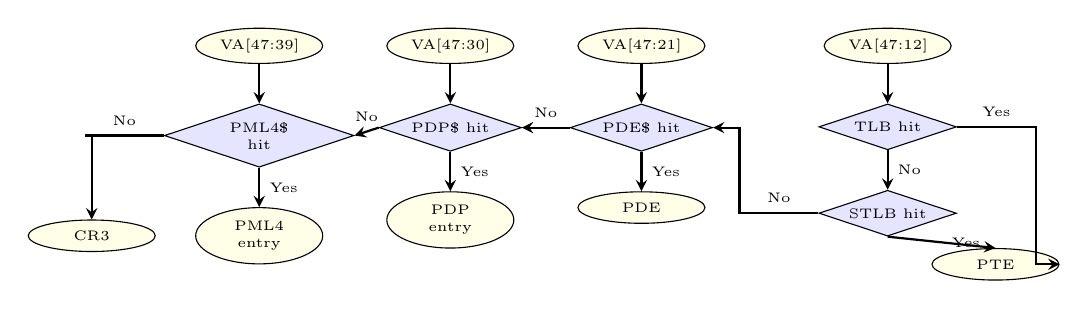
\begin{tikzpicture}[
    transform shape,
    node distance=5mm,
    decision/.style={diamond, draw, fill=blue!10, text width=1.1cm, align=center, inner sep=1pt, minimum height=0.5cm, aspect=3, font=\tiny},
    process/.style={rectangle, draw, fill=green!10, text width=2.5cm, align=center, minimum height=0.5cm, inner sep=2pt, font=\tiny},
    data/.style={ellipse, draw, fill=yellow!10, text width=1cm, align=center, minimum height=0.4cm, inner sep=2pt, font=\tiny},
    arrow/.style={->, >=stealth, thick},
    every node/.style={font=\tiny}
]

% Start
\node[data] (va) {VA[47:12]};
\node[decision, below=of va] (tlb) {TLB hit};
\node[decision, below=of tlb] (stlb) {STLB hit};
\node[data, below right=of stlb] (pte) {PTE};

\node[data, left=1.5cm of va] (va_pde) {VA[47:21]};
\node[decision, below=of va_pde] (pde_hit) {PDE\$ hit};
\node[data, below=of pde_hit] (pde) {PDE};

\node[data, left=8mm of va_pde] (va_pdp) {VA[47:30]};
\node[decision, below=of va_pdp] (pdp_hit) {PDP\$ hit};
\node[data, below=of pdp_hit] (pdp_entry) {PDP\\entry};

\node[data, left=8mm of va_pdp] (va_pml4) {VA[47:39]};
\node[decision, below=of va_pml4] (pml4_hit) {PML4\$ hit};
\node[data, below=of pml4_hit] (pml4_entry) {PML4 entry};

\node[data, left=of pml4_entry] (cr3) {CR3};

\draw[arrow] (va) -- (tlb);
\draw[arrow] (tlb) -- node[right] {No} (stlb);
\draw[arrow] (tlb.east) -- node[above] {Yes} ++(1,0) |- (pte.east);
\draw[arrow] (stlb.south) -- node[right] {Yes} (pte.north);
\draw[arrow] (stlb.west) -- node[above] {No} ++(-1,0) |- (pde_hit.east);

\draw[arrow] (va_pde) -- (pde_hit);
\draw[arrow] (pde_hit.south) -- node[right] {Yes} (pde.north);
\draw[arrow] (pde_hit.west) -- node[above] {No} (pdp_hit.east);

\draw[arrow] (va_pdp) -- (pdp_hit);
\draw[arrow] (pdp_hit.south) -- node[right] {Yes} (pdp_entry.north);
\draw[arrow] (pdp_hit.west) -- node[above] {No} (pml4_hit.east);

\draw[arrow] (va_pml4) -- (pml4_hit);
\draw[arrow] (pml4_hit.south) -- node[right] {Yes} (pml4_entry.north);
\draw[arrow] (pml4_hit.west) -- node[above] {No} ++(-1,0) -| (cr3.north);

% PML4 level
%\node[data, left=2cm of va] (va) {VA[47:21]};
%\node[decision, below=of stlb] (pml4c) {PML4\$ hit};
%\node[process, left=2.5cm of pml4c, text width=3cm, minimum height=0.8cm] (pml4load) {inject load to PML4 base + VA[47:39]×8 to get PML4 entry};
%\node[data, above=of pml4load, text width=1.3cm] (cr3) {CR3 PML4 base};
%\node[decision, below=of pml4load] (pml4l1) {L1\$ hit};
%\node[decision, below=of pml4l1] (pml4l2) {L2\$ hit};
%\node[decision, below=of pml4l2] (pml4l3) {L3\$ hit};
%\node[process, below=of pml4l3] (pml4mem) {Memory};
%\node[data, right=1cm of pml4c, text width=1.2cm] (pml4e) {PML4 entry};

% PDP level
%\node[decision, below=0.8cm of pml4c] (pdpc) {PDP\$ hit};
%\node[process, left=2.5cm of pdpc, text width=3cm, minimum height=0.8cm] (pdpload) {inject load to PDP base + VA[38:30]×8 to get PDP entry};
%\node[data, above=0.3cm of pdpload, text width=1.3cm] (pdpbase) {PDP base VA[47:39]};
%\node[decision, below=0.6cm of pdpload] (pdpl1) {L1\$ hit};
%\node[decision, below=0.4cm of pdpl1] (pdpl2) {L2\$ hit};
%\node[decision, below=0.4cm of pdpl2] (pdpl3) {L3\$ hit};
%\node[process, below=0.4cm of pdpl3] (pdpmem) {Memory};
%\node[data, right=1cm of pdpc, text width=1.2cm] (pdpe) {PDP entry};

% PDE level
%\node[decision, below=0.8cm of pdpc] (pdec) {PDE\$ hit};
%\node[process, left=2.5cm of pdec, text width=3cm, minimum height=0.8cm] (pdeload) {inject load to PDE base + VA[29:21]×8 to get PDE};
%\node[data, above=0.3cm of pdeload, text width=1.3cm] (pdebase) {PDE base VA[47:30]};
%\node[decision, below=0.6cm of pdeload] (pdel1) {L1\$ hit};
%\node[decision, below=0.4cm of pdel1] (pdel2) {L2\$ hit};
%\node[decision, below=0.4cm of pdel2] (pdel3) {L3\$ hit};
%\node[process, below=0.4cm of pdel3] (pdemem) {Memory};
%\node[data, right=1cm of pdec, text width=1.3cm] (pdee) {PDE VA[47:21]};

% PT level
%\node[process, below=1cm of pdec, text width=3cm, minimum height=0.8cm] (ptload) {inject load to PT base + VA[20:12]×8 to get PTE};
%\node[data, left=0.3cm of ptload, text width=1cm] (ptbase) {PT base};
%\node[decision, below=0.6cm of ptload] (ptl1) {L1\$ hit};
%\node[decision, below=0.4cm of ptl1] (ptl2) {L2\$ hit};
%\node[decision, below=0.4cm of ptl2] (ptl3) {L3\$ hit};
%\node[process, below=0.4cm of ptl3] (ptmem) {Memory};

% Arrows
%\draw[arrow] (va) -- (tlb);
%\draw[arrow] (tlb) -- node[right] {No} (stlb);
%\draw[arrow] (tlb.east) -- node[above] {Yes} ++(1,0) |- (pte);
%\draw[arrow] (stlb.east) -- node[above] {Yes} ++(0.8,0) |- (pte);
%\draw[arrow] (stlb) -- node[right] {No} (pml4c);

% PML4 arrows
%\draw[arrow] (pml4c) -- node[above] {No} (pml4load);
%\draw[arrow] (cr3) -- (pml4load);
%\draw[arrow] (pml4load) -- (pml4l1);
%\draw[arrow] (pml4l1) -- node[right] {No} (pml4l2);
%\draw[arrow] (pml4l2) -- node[right] {No} (pml4l3);
%\draw[arrow] (pml4l3) -- node[right] {No} (pml4mem);
%\draw[arrow] (pml4c) -- node[above] {Yes} (pml4e);
%\draw[arrow] (pml4e) -- (pdpc);
%\foreach \x in {pml4l1,pml4l2,pml4l3,pml4mem} {
%    \draw[arrow] (\x.east) -| ([xshift=0.5cm]\x.east |- pml4e) -- (pml4e);
%}

% PDP arrows
%\draw[arrow] (pdpc) -- node[above] {No} (pdpload);
%\draw[arrow] (pdpbase) -- (pdpload);
%\draw[arrow] (pdpload) -- (pdpl1);
%\draw[arrow] (pdpl1) -- node[right] {No} (pdpl2);
%\draw[arrow] (pdpl2) -- node[right] {No} (pdpl3);
%\draw[arrow] (pdpl3) -- node[right] {No} (pdpmem);
%\draw[arrow] (pdpc) -- node[above] {Yes} (pdpe);
%\draw[arrow] (pdpe) -- (pdec);
%\foreach \x in {pdpl1,pdpl2,pdpl3,pdpmem} {
%    \draw[arrow] (\x.east) -| ([xshift=0.5cm]\x.east |- pdpe) -- (pdpe);
%}

% PDE arrows
%\draw[arrow] (pdec) -- node[above] {No} (pdeload);
%\draw[arrow] (pdebase) -- (pdeload);
%\draw[arrow] (pdeload) -- (pdel1);
%\draw[arrow] (pdel1) -- node[right] {No} (pdel2);
%\draw[arrow] (pdel2) -- node[right] {No} (pdel3);
%\draw[arrow] (pdel3) -- node[right] {No} (pdemem);
%\draw[arrow] (pdec) -- node[above] {Yes} (pdee);
%\draw[arrow] (pdee) -- (ptload);
%\foreach \x in {pdel1,pdel2,pdel3,pdemem} {
%    \draw[arrow] (\x.east) -| ([xshift=0.5cm]\x.east |- pdee) -- (pdee);
%}

% PT arrows
%\draw[arrow] (ptbase) -- (ptload);
%\draw[arrow] (ptload) -- (ptl1);
%\draw[arrow] (ptl1) -- node[right] {No} (ptl2);
%\draw[arrow] (ptl2) -- node[right] {No} (ptl3);
%\draw[arrow] (ptl3) -- node[right] {No} (ptmem);
%\foreach \x in {ptl1,ptl2,ptl3,ptmem} {
%    \draw[arrow] (\x.east) -| ++(3,0) |- (pte);
%}

\end{tikzpicture}
\end{frame}

\begin{frame}{Translation Page Not Present}
\textbf{During a page walk, a translation hierarchy may return an entry with Present = 0}
\begin{itemize}
\item The page of translations pointed by this entry is not present in memory
\item PMH gets a page fault $\rightarrow$ the original load (not the PMH-injected load) faults to the OS
\item OS gets the missing translation page into memory
\item The load is re-fetched (and the PMH performs the walk again)
    \begin{itemize}
    \item The OS uses unused bits in the entry to encode the page location in the disk
    \item Most likely the lower pages in the hierarchy are also not be present
    \item OS brings all missing pages as part handling the same page fault
    \end{itemize}
\end{itemize}

\textbf{CR3 does not have a "present" bit}
\begin{itemize}
\item The PML4 table, which uses a single 4K page, is always present
\end{itemize}
\end{frame}

\begin{frame}{Cache and Translation Structures}
\begin{center}
[Diagram showing Core with PMH, L1 I\$ 32KB 8 ways, L1 D\$ 32KB 8 ways, MLC 256KB 4 ways, LLC 2MB per core, DRAM 8GB, and various TLB structures]
\end{center}
\end{frame}

% Additional advanced topics
\begin{frame}{ASID: Address Space Identifiers in TLBs}
\begin{columns}[T]
\begin{column}{0.48\textwidth}
\textbf{Problem:} TLB flush on context switch
\begin{itemize}
\item Lose all cached translations
\item Cold TLB after switch
\end{itemize}

\textbf{Solution: Address Space ID (ASID)}
\begin{itemize}
\item Unique identifier per address space
\item Tags TLB entries with process context
\item Multiple processes coexist in TLB
\item x86: called PCID, 12-bit stored in CR3[11:0]
\end{itemize}

\textbf{CR3 with ASID (CR4.PCIDE=1):}
\begin{center}
\begin{tikzpicture}[scale=0.7]
    % CR3 register
    \draw[thick] (0,0) rectangle (6,0.5);
    \fill[blue!20] (0,0) rectangle (0.8,0.5);
    \fill[green!20] (0.8,0) rectangle (5.2,0.5);
    
    % Bit positions
    \node[above, font=\tiny] at (0,0.5) {63};
    \node[above, font=\tiny] at (0.8,0.5) {12 11};
    \node[above, font=\tiny] at (6,0.5) {0};
    
    % Labels
    \node[font=\tiny] at (0.4,0.25) {NF};
    \node[font=\tiny] at (3,0.25) {PML4 Base (4KB aligned)};
    \node[font=\tiny] at (5.6,0.25) {ASID};
    
    % ASID breakdown
    \draw[thick] (4.8,-0.3) rectangle (6,-0.8);
    \foreach \i in {0,...,11} {
        \pgfmathsetmacro\x{4.8 + \i*0.1}
        \draw (\x,-0.3) -- (\x,-0.8);
    }
    \node[below, font=\tiny] at (5.4,-0.8) {12-bit ASID (PCID)}
    \draw[->] (5.4,0) -- (5.4,-0.3);
\end{tikzpicture}
\end{center}

\textbf{Software impact:}
\begin{itemize}
\item OS manages 4096 ASID values
\item Linux KPTI: separate user/kernel ASIDs
\item Critical for Meltdown mitigation
\end{itemize}
\end{column}

\begin{column}{0.52\textwidth}
\textbf{How ASID works:}
\begin{itemize}
\item TLB entries tagged with ASID
\item Lookup requires both VA match AND ASID match
\item Set-associative structure remains same
\item Parallel comparison for performance
\end{itemize}

\textbf{Key benefits:}
\begin{itemize}
\item No flush on context switch
\item Multiple address spaces in TLB
\item Reduces cold start penalty
\item Essential for virtualization
\end{itemize}
\end{column}
\end{columns}
\end{frame}

\begin{frame}{TLB Lookup with ASID}
\begin{center}
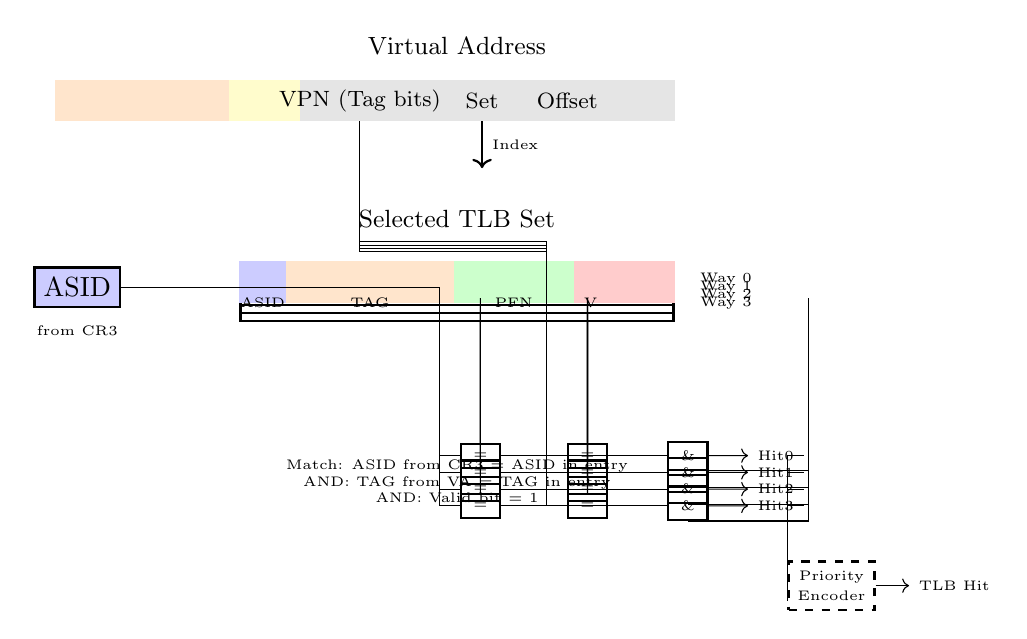
\begin{tikzpicture}[scale=0.85]
    % Define the center as reference
    \coordinate (center) at (0,0);
    
    % Virtual address at top center
    \node[rectangle, draw, thick, minimum width=5.5cm, minimum height=0.5cm, anchor=north] 
        (vaddr) at ([yshift=2.5cm]center) {};
    \fill[orange!20] ([xshift=-2.75cm]vaddr.south west) rectangle ([xshift=-0.15cm]vaddr.south west |- vaddr.north);
    \fill[yellow!20] ([xshift=-0.15cm]vaddr.south west) rectangle ([xshift=0.9cm]vaddr.south west |- vaddr.north);
    \fill[gray!20] ([xshift=0.9cm]vaddr.south west) rectangle (vaddr.north east);
    
    \node[font=\footnotesize] at ([xshift=-1.45cm]vaddr.center) {VPN (Tag bits)};
    \node[font=\footnotesize] at ([xshift=0.375cm]vaddr.center) {Set};
    \node[font=\footnotesize] at ([xshift=1.65cm]vaddr.center) {Offset};
    \node[above=2mm of vaddr, font=\small] {Virtual Address};
    
    % Arrow for set indexing
    \draw[->, thick] ([xshift=0.375cm]vaddr.south) -- ++(0,-0.7) node[midway, right, font=\tiny] {Index};
    
    % TLB Set label
    \node[below=1cm of vaddr, font=\small] (tlblabel) {Selected TLB Set};
    
    % TLB entries (4 ways) - positioned relative to label
    \foreach \way in {0,...,3} {
        \node[rectangle, draw, thick, minimum width=5.5cm, minimum height=0.45cm, 
              below={\way*0.1cm+0.3cm} of tlblabel.south, anchor=north] (entry\way) {};
        
        % ASID field
        \fill[blue!20] ([xshift=0cm]entry\way.west) rectangle ([xshift=0.7cm]entry\way.west |- entry\way.north);
        \node[font=\tiny] at ([xshift=0.35cm]entry\way.west) {ASID};
        
        % TAG field
        \fill[orange!20] ([xshift=0.7cm]entry\way.west) rectangle ([xshift=3.2cm]entry\way.west |- entry\way.north);
        \node[font=\tiny] at ([xshift=1.95cm]entry\way.west) {TAG};
        
        % PFN field
        \fill[green!20] ([xshift=3.2cm]entry\way.west) rectangle ([xshift=5cm]entry\way.west |- entry\way.north);
        \node[font=\tiny] at ([xshift=4.1cm]entry\way.west) {PFN};
        
        % Valid bit
        \fill[red!20] ([xshift=5cm]entry\way.west) rectangle (entry\way.east |- entry\way.north);
        \node[font=\tiny] at ([xshift=5.25cm]entry\way.west) {V};
        
        % Way label
        \node[right=2mm of entry\way, font=\tiny] {Way \way};
    }
    
    % CR3 ASID source - positioned left of TLB entries
    \node[rectangle, draw, thick, fill=blue!20, minimum width=1cm, minimum height=0.5cm,
          left=1.5cm of entry1.west] (cr3asid) {ASID};
    \node[below=1mm of cr3asid, font=\tiny] {from CR3};
    
    % Comparison logic below TLB entries
    \coordinate (compbase) at ([yshift=-2cm]entry3.south);
    
    \foreach \way in {0,...,3} {
        % ASID comparator
        \node[rectangle, draw, thick, minimum width=0.5cm, minimum height=0.15cm,
              at={([xshift=0.35cm, yshift={\way*-0.25cm}]compbase)}] (asidcmp\way) {\tiny =};
        
        % TAG comparator
        \node[rectangle, draw, thick, minimum width=0.5cm, minimum height=0.15cm,
              at={([xshift=1.95cm, yshift={\way*-0.25cm}]compbase)}] (tagcmp\way) {\tiny =};
        
        % AND gate
        \node[rectangle, draw, thick, minimum width=0.5cm, minimum height=0.15cm,
              at={([xshift=3.45cm, yshift={\way*-0.25cm}]compbase)}] (and\way) {\tiny \&};
        
        % Connections from TLB entries
        \draw[-] ([xshift=0.35cm]entry\way.south) -- (asidcmp\way.north);
        \draw[-] ([xshift=1.95cm]entry\way.south) -- (tagcmp\way.north);
        
        % Connection from CR3 ASID
        \draw[-] (cr3asid.east) -| ([xshift=-0.3cm]asidcmp\way.west) -- (asidcmp\way.west);
        
        % Connection from VA TAG
        \draw[-] ([xshift=-1.45cm]vaddr.south) -- ([xshift=-1.45cm, yshift=-1.8cm-\way*0.05cm]vaddr.south) 
                 -| ([xshift=-0.3cm]tagcmp\way.west) -- (tagcmp\way.west);
        
        % Connect comparators to AND
        \draw[-] (asidcmp\way.east) -- (and\way.west);
        \draw[-] (tagcmp\way.east) -- (and\way.west);
        
        % Valid bit check
        \draw[-] ([xshift=5.25cm]entry\way.south) |- (and\way.south);
        
        % Hit output
        \node[right=5mm of and\way] (hit\way) {\tiny Hit\way};
        \draw[->] (and\way.east) -- (hit\way.west);
    }
    
    % Priority encoder
    \node[rectangle, draw, thick, dashed, minimum width=0.8cm, minimum height=0.6cm,
          below right=0.5cm and 1cm of and3] (encoder) {\tiny \shortstack{Priority\\Encoder}};
    
    % Hit signals to encoder
    \foreach \way in {0,...,3} {
        \draw[-] (hit\way.east) -| ([yshift={\way*0.15cm-0.225cm}]encoder.west);
    }
    
    % Final TLB Hit
    \draw[->] (encoder.east) -- ++(0.5,0) node[right, font=\tiny] {TLB Hit};
    
    % Bottom caption
    \node[font=\tiny, align=center] at ([yshift=-3.5cm]center) {
        Match: ASID from CR3 = ASID in entry\\
        AND: TAG from VA = TAG in entry\\
        AND: Valid bit = 1
    };
\end{tikzpicture}
\end{center}
\end{frame}

\begin{frame}{Contiguous PTE (ContPTE) - ARM Feature}
\begin{columns}[T]
\begin{column}{0.45\textwidth}
\textbf{Problem:} TLB pressure
\begin{itemize}
\item One TLB entry per 4KB page
\item Large regions → many TLB entries
\item 2MB pages often too large
\end{itemize}

\textbf{ContPTE Solution:}
\begin{itemize}
\item 16 consecutive PTEs marked "contiguous"
\item Maps 64KB (16 × 4KB)
\item Hardware coalesces into single TLB entry
\end{itemize}

\textbf{Requirements:}
\begin{itemize}
\item Physical pages must be contiguous
\item Same permissions for all 16 pages
\item Contiguous bit set in all 16 PTEs
\end{itemize}

\textbf{Benefits:}
\begin{itemize}
\item 16× TLB reach improvement
\item No page table format changes
\item Transparent to applications
\end{itemize}
\end{column}

\begin{column}{0.55\textwidth}
\textbf{Page Table with ContPTE:}
\begin{center}
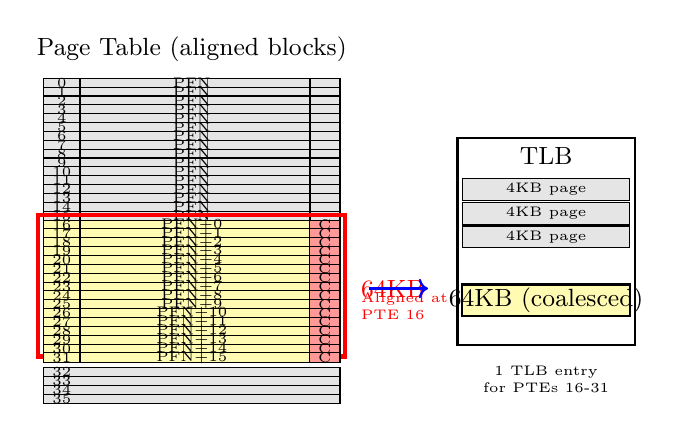
\begin{tikzpicture}[scale=0.75]
    % Page table entries
    \node[font=\small] at (2.5,4.5) {Page Table (aligned blocks)};
    
    % Draw some regular PTEs (0-15)
    \foreach \i in {0,...,15} {
        \pgfmathsetmacro\y{4 - \i*0.15}
        \draw[thick] (0,\y) rectangle (5,\y-0.14);
        \fill[gray!20] (0,\y) rectangle (5,\y-0.14);
        \node[font=\tiny] at (0.3,\y-0.07) {\i};
        % Show PFN and flags more abstractly
        \draw[thick] (0.6,\y) -- (0.6,\y-0.14);
        \draw[thick] (4.5,\y) -- (4.5,\y-0.14);
        \node[font=\tiny] at (2.5,\y-0.07) {PFN};
    }
    
    % Naturally aligned contiguous block (16 entries starting at PTE 16)
    \draw[thick, red, line width=1.5pt] (-0.1,1.7) rectangle (5.1,-0.7);
    \foreach \i in {0,...,15} {
        \pgfmathsetmacro\idx{int(\i + 16)}
        \pgfmathsetmacro\y{1.6 - \i*0.15}
        \draw[thick] (0,\y) rectangle (5,\y-0.14);
        \fill[yellow!30] (0,\y) rectangle (5,\y-0.14);
        
        % PTE number
        \node[font=\tiny] at (0.3,\y-0.07) {\idx};
        \draw[thick] (0.6,\y) -- (0.6,\y-0.14);
        
        % Physical frame - show they're contiguous
        \pgfmathsetmacro\pfn{int(1000 + \i)}
        \node[font=\tiny] at (2.5,\y-0.07) {PFN+\i};
        
        % Contiguous bit
        \draw[thick] (4.5,\y) -- (4.5,\y-0.14);
        \fill[red!40] (4.5,\y) rectangle (5,\y-0.14);
        \node[font=\tiny] at (4.75,\y-0.07) {C};
    }
    
    % More regular PTEs after
    \foreach \i in {32,...,35} {
        \pgfmathsetmacro\idx{int(\i - 32)}
        \pgfmathsetmacro\y{-0.9 - \idx*0.15}
        \draw[thick] (0,\y) rectangle (5,\y-0.14);
        \fill[gray!20] (0,\y) rectangle (5,\y-0.14);
        \node[font=\tiny] at (0.3,\y-0.07) {\i};
    }
    
    % Label for contiguous block
    \node[right, font=\small, red] at (5.2,0.45) {64KB};
    \node[right, font=\tiny, red, align=left] at (5.2,0.15) {Aligned at\\PTE 16};
    
    % Arrow showing coalescing
    \draw[->, thick, blue] (5.5,0.45) -- (6.5,0.45);
    
    % TLB representation
    \draw[thick] (7,-0.5) rectangle (10,3);
    \node[font=\small] at (8.5,2.7) {TLB};
    
    % Regular entries
    \foreach \i in {0,1,2} {
        \pgfmathsetmacro\y{2.3 - \i*0.4}
        \draw[thick] (7.1,\y) rectangle (9.9,\y-0.35);
        \fill[gray!20] (7.1,\y) rectangle (9.9,\y-0.35);
        \node[font=\tiny] at (8.5,\y-0.175) {4KB page};
    }
    
    % Coalesced entry
    \draw[thick, line width=1.5pt] (7.1,0.5) rectangle (9.9,0);
    \fill[yellow!30] (7.1,0.5) rectangle (9.9,0);
    \node[font=\small] at (8.5,0.25) {64KB (coalesced)};
    
    % Annotation
    \node[below, font=\tiny, align=center] at (8.5,-0.7) {1 TLB entry\\for PTEs 16-31};
\end{tikzpicture}
\end{center}
\end{column}
\end{columns}
\end{frame}

\begin{frame}{ContPTE: TLB Lookup Mechanism}
\begin{center}
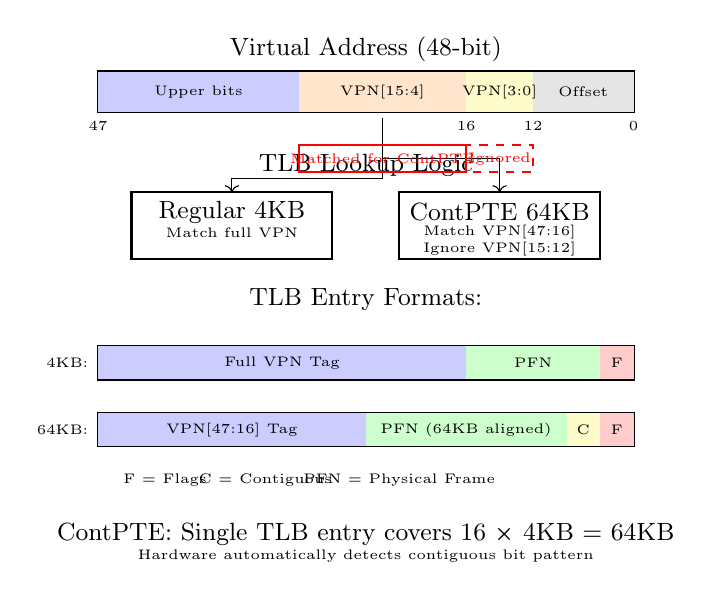
\begin{tikzpicture}[scale=0.85]
    % Virtual Address
    \draw[thick] (0,6) rectangle (8,6.6);
    \node[above, font=\small] at (4,6.6) {Virtual Address (48-bit)};
    
    % VA fields
    \fill[blue!20] (0,6) rectangle (3,6.6);
    \fill[orange!20] (3,6) rectangle (5.5,6.6);
    \fill[yellow!20] (5.5,6) rectangle (6.5,6.6);
    \fill[gray!20] (6.5,6) rectangle (8,6.6);
    
    \node[font=\tiny] at (1.5,6.3) {Upper bits};
    \node[font=\tiny] at (4.25,6.3) {VPN[15:4]};
    \node[font=\tiny] at (6,6.3) {VPN[3:0]};
    \node[font=\tiny] at (7.25,6.3) {Offset};
    
    % Bit positions
    \node[below, font=\tiny] at (0,6) {47};
    \node[below, font=\tiny] at (5.5,6) {16};
    \node[below, font=\tiny] at (6.5,6) {12};
    \node[below, font=\tiny] at (8,6) {0};
    
    % TLB lookup paths
    \node[font=\small] at (4,5.2) {TLB Lookup Logic};
    
    % Regular 4KB lookup
    \draw[thick] (0.5,4.8) rectangle (3.5,3.8);
    \node[font=\small] at (2,4.5) {Regular 4KB};
    \node[font=\tiny] at (2,4.2) {Match full VPN};
    \draw[->] (4.25,5.9) -- (4.25,5) -- (2,5) -- (2,4.8);
    
    % ContPTE 64KB lookup
    \draw[thick] (4.5,4.8) rectangle (7.5,3.8);
    \node[font=\small] at (6,4.5) {ContPTE 64KB};
    \node[font=\tiny] at (6,4.2) {Match VPN[47:16]};
    \node[font=\tiny] at (6,3.95) {Ignore VPN[15:12]};
    \draw[->] (4.25,5.9) -- (4.25,5.3) -- (6,5.3) -- (6,4.8);
    
    % Show which bits are matched
    \draw[thick, red] (3,5.5) rectangle (5.5,5.1);
    \node[font=\tiny, red] at (4.25,5.3) {Matched for ContPTE};
    
    \draw[thick, dashed, red] (5.5,5.5) rectangle (6.5,5.1);
    \node[font=\tiny, red] at (6,5.3) {Ignored};
    
    % TLB entry format
    \node[font=\small] at (4,3.2) {TLB Entry Formats:};
    
    % 4KB entry
    \draw[thick] (0,2.5) rectangle (8,2);
    \fill[blue!20] (0,2.5) rectangle (5.5,2);
    \fill[green!20] (5.5,2.5) rectangle (7.5,2);
    \fill[red!20] (7.5,2.5) rectangle (8,2);
    \node[font=\tiny] at (2.75,2.25) {Full VPN Tag};
    \node[font=\tiny] at (6.5,2.25) {PFN};
    \node[font=\tiny] at (7.75,2.25) {F};
    \node[left, font=\tiny] at (0,2.25) {4KB:};
    
    % 64KB entry
    \draw[thick] (0,1.5) rectangle (8,1);
    \fill[blue!20] (0,1.5) rectangle (4,1);
    \fill[green!20] (4,1.5) rectangle (7,1);
    \fill[yellow!20] (7,1.5) rectangle (7.5,1);
    \fill[red!20] (7.5,1.5) rectangle (8,1);
    \node[font=\tiny] at (2,1.25) {VPN[47:16] Tag};
    \node[font=\tiny] at (5.5,1.25) {PFN (64KB aligned)};
    \node[font=\tiny] at (7.25,1.25) {C};
    \node[font=\tiny] at (7.75,1.25) {F};
    \node[left, font=\tiny] at (0,1.25) {64KB:};
    
    % Legend
    \node[font=\tiny] at (1,0.5) {F = Flags};
    \node[font=\tiny] at (2.5,0.5) {C = Contiguous};
    \node[font=\tiny] at (4.5,0.5) {PFN = Physical Frame};
    
    % Bottom note
    \node[below, font=\small, align=center] at (4,0) {ContPTE: Single TLB entry covers 16 × 4KB = 64KB};
    \node[below, font=\tiny, align=center] at (4,-0.4) {Hardware automatically detects contiguous bit pattern};
\end{tikzpicture}
\end{center}
\end{frame}

\begin{frame}{TLB Shootdown: Maintaining Coherency}
\begin{columns}[T]
\begin{column}{0.55\textwidth}
\textbf{Problem: TLB coherency across cores}
\begin{itemize}
\item CPU 0 unmaps a page
\item CPU 1's TLB still has old mapping
\item Can access freed/reused memory!
\end{itemize}

\textbf{Classic TLB Shootdown (IPI-based):}
\begin{enumerate}
\item Initiator updates page table
\item Send Inter-Processor Interrupt to all CPUs
\item Each CPU invalidates TLB entry
\item Wait for all acknowledgments
\item Continue execution
\end{enumerate}

\textbf{Performance impact:}
\begin{itemize}
\item Synchronous operation - initiator waits
\item IPIs interrupt all CPUs
\item Scales poorly with core count
\end{itemize}
\end{column}

\begin{column}{0.45\textwidth}
\begin{center}
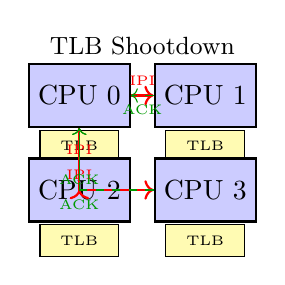
\begin{tikzpicture}[scale=0.8]
    % CPU cores
    \foreach \i in {0,1,2,3} {
        \node[rectangle, draw, thick, minimum width=1.2cm, minimum height=0.8cm, fill=blue!20] 
            (cpu\i) at ({mod(\i,2)*2}, {-floor(\i/2)*1.5}) {CPU \i};
        \node[rectangle, draw, minimum width=1cm, minimum height=0.4cm, fill=yellow!30] 
            (tlb\i) at ({mod(\i,2)*2}, {-floor(\i/2)*1.5-0.8}) {\tiny TLB};
    }
    
    % IPI arrows from CPU 0
    \draw[->, thick, red] (cpu0) -- node[above, sloped] {\tiny IPI} (cpu1);
    \draw[->, thick, red] (cpu0) |- node[near end, above] {\tiny IPI} (cpu2);
    \draw[->, thick, red] (cpu0) |- node[pos=0.3, above] {\tiny IPI} (cpu3);
    
    % ACK arrows back
    \draw[->, dashed, green!60!black] (cpu1) -- node[below, sloped] {\tiny ACK} (cpu0);
    \draw[->, dashed, green!60!black] (cpu2) -| node[near start, below] {\tiny ACK} (cpu0);
    \draw[->, dashed, green!60!black] (cpu3) -| node[pos=0.7, below] {\tiny ACK} (cpu0);
    
    \node[above] at (1, 0.5) {\small TLB Shootdown};
\end{tikzpicture}
\end{center}

\textbf{Software workarounds:}
\begin{itemize}
\item Batch multiple invalidations
\item Lazy TLB mode for idle CPUs
\item Per-CPU page tables (KPTI)
\end{itemize}
\end{column}
\end{columns}
\end{frame}

\begin{frame}{Modern TLB Invalidation: Broadcast Instructions}
\begin{columns}[T]
\begin{column}{0.55\textwidth}
\textbf{INVLPGB (AMD) / TLBSYNC:}
\begin{itemize}
\item Broadcast invalidation without IPIs
\item Hardware handles coherency protocol
\item Non-blocking for initiator
\end{itemize}

\textbf{How it works:}
\begin{enumerate}
\item Execute INVLPGB with address range
\item Hardware broadcasts to all cores
\item TLBSYNC waits for completion
\item Can continue other work between INVLPGB and TLBSYNC
\end{enumerate}

\textbf{ARM: TLBI with broadcast}
\begin{itemize}
\item TLBI instructions with Inner Shareable scope
\item Automatic broadcast to all cores in domain
\item No software IPIs needed
\end{itemize}
\end{column}

\begin{column}{0.45\textwidth}
\begin{center}
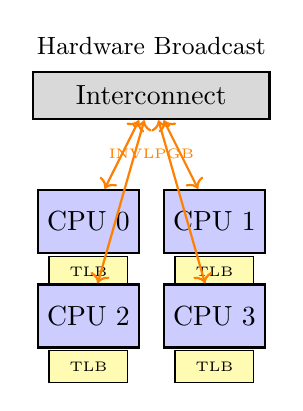
\begin{tikzpicture}[scale=0.8]
    % Memory controller/interconnect
    \node[rectangle, draw, thick, minimum width=3cm, minimum height=0.6cm, fill=gray!30] 
        (interconnect) at (1, 0.5) {Interconnect};
    
    % CPU cores
    \foreach \i in {0,1,2,3} {
        \node[rectangle, draw, thick, minimum width=1.2cm, minimum height=0.8cm, fill=blue!20] 
            (cpu\i) at ({mod(\i,2)*2}, {-floor(\i/2)*1.5-1.5}) {CPU \i};
        \node[rectangle, draw, minimum width=1cm, minimum height=0.4cm, fill=yellow!30] 
            (tlb\i) at ({mod(\i,2)*2}, {-floor(\i/2)*1.5-2.3}) {\tiny TLB};
        
        % Hardware broadcast lines
        \draw[<->, thick, orange] (cpu\i) -- (interconnect);
    }
    
    % Broadcast indication
    \node[above] at (1, 1) {\small Hardware Broadcast};
    \node[text=orange, below] at (1, -0.2) {\tiny INVLPGB};
\end{tikzpicture}
\end{center}

\textbf{Software benefits:}
\begin{itemize}
\item No IPI overhead
\item Better scalability with core count
\item Asynchronous operation possible
\item Lower latency for munmap(), mprotect()
\end{itemize}

\textbf{When you see the impact:}
\begin{itemize}
\item JVM garbage collectors (unmapping large heaps)
\item Database buffer pool resizing
\item Container memory limits changes
\end{itemize}
\end{column}
\end{columns}
\end{frame}

\begin{frame}{Software Impact: When These Features Matter}
\begin{itemize}
\item \textbf{ASID helps when:}
    \begin{itemize}
    \item Many short-lived processes (web servers, shell scripts)
    \item Frequent system calls with KPTI/Meltdown mitigation
    \item Container workloads with namespace switches
    \end{itemize}
    
\item \textbf{ContPTE/THP benefits:}
    \begin{itemize}
    \item Large memory allocations (databases, scientific computing)
    \item Better than nothing when huge pages fragment
    \item mmap() with MAP\_POPULATE for large files
    \end{itemize}
    
\item \textbf{TLB shootdown overhead visible in:}
    \begin{itemize}
    \item fork()/exit() in multithreaded programs
    \item Memory-mapped file operations across threads
    \item Dynamic memory allocators (malloc/free of large chunks)
    \item Live migration of VMs
    \end{itemize}
    
\item \textbf{Performance monitoring:}
    \begin{itemize}
    \item \texttt{perf stat -e tlb:tlb\_flush} - count TLB flushes
    \item \texttt{/proc/interrupts} - look for TLB shootdown IPIs
    \item High system CPU time often indicates TLB management overhead
    \end{itemize}
\end{itemize}
\end{frame}

% Backup slides section
\section{Backup}

\begin{frame}{Backup}
\begin{center}
\Huge Backup
\end{center}
\end{frame}

\begin{frame}{Why Virtual Memory?}
\begin{itemize}
\item \textbf{Generality} – ability to run programs larger than size of physical memory
\item \textbf{Storage management} – allocation/deallocation of variable sized blocks is costly and leads to (external) fragmentation
\item \textbf{Protection} – regions of the address space can be R/O, Ex, ...
\item \textbf{Flexibility} – portions of a program can be placed anywhere, without relocation
\item \textbf{Storage efficiency} – retain only most important portions of the program in memory
\item \textbf{Concurrent I/O} – execute other processes while loading/dumping page
\item \textbf{Expandability} – can leave room in virtual address space for objects to grow
\item \textbf{Performance}
\end{itemize}
\end{frame}

\begin{frame}{Page Aliasing}
\textbf{OS may map different virtual pages to the same physical page}

\textbf{DLLs in Linux/Windows}
\begin{itemize}
\item DLL pages are used by all processes, marked as read only
\item Same DLL may be loaded by a process more than once
\end{itemize}

\textbf{Large malloc – Copy-on-Write}
\begin{itemize}
\item OS maps all allocated virtual pages to the same all-zero physical page
\item The newly allocated virtual page is marked as read-only in its PTE
\item In case of a write to one of these virtual pages:
    \begin{itemize}
    \item Get access violation page-fault
    \item OS identifies that the page is mapped to the special physical page
    \item OS allocates a "real" physical page (copy-on-write)
    \end{itemize}
\end{itemize}

\textbf{Shared Memory}
\begin{itemize}
\item OS maps virtual pages of different processes to the same physical page
\end{itemize}
\end{frame}

\begin{frame}{32bit Mode: 4KB Page Mapping}
\textbf{2-level hierarchical mapping}
\begin{itemize}
\item Page directory and page tables
\item Pages / page tables are 4KB aligned
\end{itemize}

\begin{itemize}
\item CR3 points to the current Page Directory
\item Upper 10 Linear addr. bits point to a PDE
    \begin{itemize}
    \item PDE provides a 20 bit, 4KB aligned base physical address of a page table
    \end{itemize}
\item Next 10 Linear addr. bits point to a PTE within the given Page Table
    \begin{itemize}
    \item PTE provides a 20 bit, 4KB aligned, base physical address of a 4KB page
    \end{itemize}
\item Lowest 12 Linear Addr. bits provide offset within the selected 4KB page
\end{itemize}
\end{frame}

\begin{frame}{32bit Mode: 4MB Page Mapping}
\begin{itemize}
\item PDE directly maps up to 1024 4MB pages
\item Upper 10 Linear addr. bits point to a PDE
    \begin{itemize}
    \item PS in the PDE = 1
    \item PDE provides a 10 bit, 4MB aligned, base physical address of a 4MB page
    \end{itemize}
\item Lowest 22 Linear addr. bits provide offset within selected 4MB page
\end{itemize}

\textbf{Mixing 4KByte and 4MByte Pages}
\begin{itemize}
\item Separate TLBs for 4MB pages and 4KB pages
    \begin{itemize}
    \item Often-used code (e.g., kernels) is placed in a 4MB page $\rightarrow$ frees up 4KB TLB entries
    \item Reduces TLB misses and improve overall system performance
    \end{itemize}
\end{itemize}
\end{frame}

\begin{frame}{PAE – Physical Address Extension}
\textbf{When PAE (physical address extension) flag in CR4 is set}
\begin{itemize}
\item Physical addresses is extended to M bits
    \begin{itemize}
    \item Linear address remains 32 bit
    \end{itemize}
\item Each page table entry becomes 64 bits to hold the extra phy. address bits
    \begin{itemize}
    \item Page directory and page tables remain 4KB in size
    \item Number of entries in each table is halved to 512
    \item Indexed by 9 instead of 10 bits
    \end{itemize}
\end{itemize}

\textbf{A new 4 entry Page Directory Pointer Table is added}
\begin{itemize}
\item Indexed by bits [31:30] of the linear address
\item Each entry points to a page directory
\item CR3 contains the page-directory-pointer-table base address
    \begin{itemize}
    \item Provides the m.s.bits of the physical address
    \item Forcing the table to be located on a 32-byte boundary
    \end{itemize}
\end{itemize}
\end{frame}

\begin{frame}{Execute-Disable Bit}
\textbf{Supported only with PAE enabled / 64 bit mode}
\begin{itemize}
\item Bit[63] in PML4 entry, PDP entry, PDE, PTE
\end{itemize}

\textbf{If the execute disable bit of a memory page is set}
\begin{itemize}
\item The page can be used only as data
\item An attempt to execute code from a memory page with the execute-disable bit set causes a page-fault exception
\item Setting the execute-disable bit at any level of the paging structure, protects all pages pointed from this entry
\end{itemize}
\end{frame}

\begin{frame}{Page Table – Virtual Mem. Attributes}
\textbf{Present (P) flag}
\begin{itemize}
\item When set: page is in physical memory
\item When clear, page not in memory $\rightarrow$ processor generates a page-fault
\item The processor does not set/clear this flag – OS maintains its state
\item In case of a page-fault, the OS performs the following operations:
    \begin{enumerate}
    \item Copy the page from disk into physical memory
    \item Load page address into PTE/PDE; set present=1, dirty=0, accessed=0
    \item Invalidate victim page from TLB
    \item Return from page-fault handler and restart the program
    \end{enumerate}
\end{itemize}

\textbf{Page size (PS) flag, in PDEs only}
\begin{itemize}
\item 0: The PDE points to a page table of 4KBytes pages
\item 1: The PDE points to a 4MB page
\end{itemize}
\end{frame}

\begin{frame}{Page Table – Virtual Mem. Attributes (cont.)}
\textbf{Accessed (A) flag and Dirty (D) flag}
\begin{itemize}
\item Typically cleared by the OS when a page/PT initially loaded into physical mem
\item Processor sets the A-flag the first time a page/PT is accessed (read/write)
\item Processor sets the D-flag the first time a page is accessed for a write
    \begin{itemize}
    \item The D-flag is not used in PDEs which point to page tables
    \end{itemize}
\item Both A and D flag are sticky
    \begin{itemize}
    \item Once set, the processor does not implicitly clear it – only software can clear it
    \end{itemize}
\item Used by OS to manage transfer of pages/PTs tables into and out of physical memory
\end{itemize}

\textbf{Global (G) flag}
\begin{itemize}
\item Indicates a global page when set (+ page global enable is set: CR4.PGE =1)
\item PTE/PDE in TLB not invalidated when CR3 is loaded / task switch
\item Only software can set or clear this flag
\end{itemize}
\end{frame}

\begin{frame}{Page Table – Caching Attributes}
\textbf{Page-level write-through (PWT) flag}
\begin{itemize}
\item Controls the write-through or write-back caching policy of the page / PT
    \begin{itemize}
    \item 0 : write-back caching, 1: write-through caching
    \end{itemize}
\item Ignored if the CD (cache disable) flag in CR0 is set
\end{itemize}

\textbf{Page-level cache disable (PCD) flag}
\begin{itemize}
\item Controls the caching of individual pages/PT
\item 1: caching of the associated page/PT is prevented
\item 0: the page/PT can be cached
\item Ignored (assumes as set) if the CD (cache disable) flag in CR0 is set
\end{itemize}

\textbf{Page table attribute index (PAT) flag}
\begin{itemize}
\item Used along with the PCD and PWT flags to select an entry in the PAT
\item Which in turn selects the memory type for the page
\end{itemize}
\end{frame}

\begin{frame}{Page Table – Protection Attributes}
\textbf{Read/write (R/W) flag}
\begin{itemize}
\item Specifies the read-write privileges for a page or group of pages
\item 0: the page is read only
\item 1: the page can be read and written into
\end{itemize}

\textbf{User/supervisor (U/S) flag}
\begin{itemize}
\item Specifies the user-supervisor privileges for a page or group of pages
\item 0: supervisor privilege level
\item 1: user privilege level
\end{itemize}
\end{frame}

\begin{frame}{Page Directory Base Address}
\textbf{The physical address of the page directory is stored in CR3 register}
\begin{itemize}
\item Also called the page directory base register (PDBR)
\end{itemize}

\textbf{PDBR is typically loaded with a new as part of a task switch}

\textbf{OS must ensure that}
\begin{itemize}
\item The page directory indicated by the PDBR image in a task's TSS (task state segment) is present in physical memory before the task is dispatched
\item The page directory must also remain in memory as long as the task is active
\end{itemize}
\end{frame}

\begin{frame}{TLBs}
\textbf{OS running at privilege level 0 can invalidate TLB entries}
\begin{itemize}
\item INVLPG instruction invalidates a specific PTE in the TLB
    \begin{itemize}
    \item This instruction ignores the setting of the G flag
    \end{itemize}
\item Whenever a PDE/PTE is changed (also when present flag is set to 0)
    \begin{itemize}
    \item OS must invalidate the corresponding TLB entry
    \end{itemize}
\item All (non-global) TLBs are automatically invalidated when CR3 is loaded
\end{itemize}

\textbf{The global (G) flag prevents frequently used pages from being automatically invalidated in on a task switch}
\begin{itemize}
\item The entry remains in the TLB indefinitely
\item Only INVLPG can invalidate a global page entry
\end{itemize}
\end{frame}

\begin{frame}{PTE/PDE/PDP/PML4 Entry Format}
\tiny
\definecolor{addrcolor}{HTML}{E6E6FA}
\definecolor{igncolor}{HTML}{FFE4E1}
\definecolor{rsvcolor}{HTML}{F0F0F0}
\definecolor{pagesizeyellow}{HTML}{FFFF00}

\begin{tikzpicture}[scale=1, transform shape]

% Bit numbers at top
\node[anchor=east] at (0.1,7.6) {\tiny 63};
\node[anchor=west] at (1.8,7.6) {\tiny 52 51};
\node[anchor=center] at (6.0,7.6) {\tiny M M-1};
\node[anchor=east] at (9.3,7.6) {\tiny 12 11};
\node[anchor=east] at (10.5,7.6) {\tiny 9 8 7 6 5 4 3 2 1 0};

% CR3 row
\draw[thick] (0,7.2) rectangle (11.4,6.4);
\fill[rsvcolor] (0,7.2) rectangle (2.1,6.4);
\fill[addrcolor] (2.1,7.2) rectangle (9.4,6.4);
\fill[igncolor] (9.4,7.2) rectangle (10.5,6.4);
\node at (1.05,6.8) {\tiny Reserved};
\node at (5.75,6.8) {\tiny Address of PML4 table};
\node at (9.95,6.8) {\tiny Ignored};
% Draw individual bit cells for flags
\foreach \x in {10.5,10.65,10.8,10.95,11.1,11.25} {
    \draw ({\x},7.2) rectangle ({\x+0.15},6.4);
}
\node[anchor=west] at (11.6,6.8) {\textbf{CR3}};

% PML4E row
\draw[thick] (0,6.4) rectangle (11.4,5.6);
\fill[igncolor] (0,6.4) rectangle (0.3,5.6);
\fill[igncolor] (0.3,6.4) rectangle (2.1,5.6);
\fill[rsvcolor] (2.1,6.4) rectangle (2.7,5.6);
\fill[addrcolor] (2.7,6.4) rectangle (9.4,5.6);
\fill[igncolor] (9.4,6.4) rectangle (9.9,5.6);
\node[rotate=90,anchor=center] at (0.15,6.0) {\tiny XD};
\node at (1.2,6.0) {\tiny Ignored};
\node at (2.4,6.0) {\tiny Rsvd.};
\node at (6.05,6.0) {\tiny Address of page-directory-pointer table};
\node at (9.65,6.0) {\tiny Ign.};
% Individual flag bits
\foreach \x in {9.9,10.05,10.2,10.35,10.5,10.65,10.8,10.95,11.1,11.25} {
    \draw ({\x},6.4) rectangle ({\x+0.15},5.6);
}
\node[rotate=90,anchor=center] at (10.125,6.0) {\tiny A};
\node[rotate=90,anchor=center] at (10.575,6.0) {\tiny PCD};
\node[rotate=90,anchor=center] at (10.725,6.0) {\tiny PWT};
\node[rotate=90,anchor=center] at (10.875,6.0) {\tiny US};
\node[rotate=90,anchor=center] at (11.025,6.0) {\tiny RW};
\node[rotate=90,anchor=center] at (11.175,6.0) {\tiny P};
\node[anchor=west] at (11.6,6.2) {\textbf{PML4E:}};
\node[anchor=west] at (11.6,5.8) {\textbf{present}};

% PDPTE 1GB row
\draw[thick] (0,5.6) rectangle (11.4,4.8);
\fill[igncolor] (0,5.6) rectangle (0.3,4.8);
\fill[igncolor] (0.3,5.6) rectangle (2.1,4.8);
\fill[rsvcolor] (2.1,5.6) rectangle (2.7,4.8);
\fill[addrcolor] (2.7,5.6) rectangle (5.8,4.8);
\fill[rsvcolor] (5.8,5.6) rectangle (9.4,4.8);
\fill[igncolor] (9.4,5.6) rectangle (9.75,4.8);
\node[rotate=90,anchor=center] at (0.15,5.2) {\tiny XD};
\node at (1.2,5.2) {\tiny Ignored};
\node at (2.4,5.2) {\tiny Rsvd.};
\node at (4.25,5.2) {\tiny\begin{tabular}{c}Address of\\1GB page frame\end{tabular}};
\node at (7.6,5.2) {\tiny Reserved};
\node at (9.575,5.2) {\tiny Ign.};
% Individual flag bits
\foreach \x in {9.75,9.9,10.05,10.2,10.35,10.5,10.65,10.8,10.95,11.1,11.25} {
    \draw ({\x},5.6) rectangle ({\x+0.15},4.8);
}
\fill[pagesizeyellow] (10.35,5.6) rectangle (10.5,4.8);
\node[rotate=90,anchor=center] at (9.825,5.2) {\tiny G};
\node[rotate=90,anchor=center] at (10.125,5.2) {\tiny DA};
\node[rotate=90,anchor=center] at (10.275,5.2) {\tiny A};
\node[rotate=90,anchor=center] at (10.425,5.2) {\tiny 1};
\node[rotate=90,anchor=center] at (10.575,5.2) {\tiny PCD};
\node[rotate=90,anchor=center] at (10.725,5.2) {\tiny PWT};
\node[rotate=90,anchor=center] at (10.875,5.2) {\tiny US};
\node[rotate=90,anchor=center] at (11.025,5.2) {\tiny RW};
\node[rotate=90,anchor=center] at (11.175,5.2) {\tiny P};
\node[anchor=west] at (11.6,5.4) {\textbf{PDPTE:}};
\node[anchor=west] at (11.6,5.2) {\textbf{1GB}};
\node[anchor=west] at (11.6,5.0) {\textbf{page}};

% PDPTE page directory row
\draw[thick] (0,4.8) rectangle (11.4,4.0);
\fill[igncolor] (0,4.8) rectangle (0.3,4.0);
\fill[igncolor] (0.3,4.8) rectangle (2.1,4.0);
\fill[rsvcolor] (2.1,4.8) rectangle (2.7,4.0);
\fill[addrcolor] (2.7,4.8) rectangle (9.4,4.0);
\fill[igncolor] (9.4,4.8) rectangle (9.9,4.0);
\node[rotate=90,anchor=center] at (0.15,4.4) {\tiny XD};
\node at (1.2,4.4) {\tiny Ignored};
\node at (2.4,4.4) {\tiny Rsvd.};
\node at (6.05,4.4) {\tiny Address of page directory};
\node at (9.65,4.4) {\tiny Ign.};
% Individual flag bits
\foreach \x in {9.9,10.05,10.2,10.35,10.5,10.65,10.8,10.95,11.1,11.25} {
    \draw ({\x},4.8) rectangle ({\x+0.15},4.0);
}
\fill[pagesizeyellow] (10.35,4.8) rectangle (10.5,4.0);
\node[rotate=90,anchor=center] at (10.125,4.4) {\tiny A};
\node[rotate=90,anchor=center] at (10.425,4.4) {\tiny 0};
\node[rotate=90,anchor=center] at (10.575,4.4) {\tiny PCD};
\node[rotate=90,anchor=center] at (10.725,4.4) {\tiny PWT};
\node[rotate=90,anchor=center] at (10.875,4.4) {\tiny US};
\node[rotate=90,anchor=center] at (11.025,4.4) {\tiny RW};
\node[rotate=90,anchor=center] at (11.175,4.4) {\tiny P};
\node[anchor=west] at (11.6,4.6) {\textbf{PDPTE:}};
\node[anchor=west] at (11.6,4.4) {\textbf{page}};
\node[anchor=west] at (11.6,4.2) {\textbf{directory}};

% PDE 2MB row
\draw[thick] (0,4.0) rectangle (11.4,3.2);
\fill[igncolor] (0,4.0) rectangle (0.3,3.2);
\fill[igncolor] (0.3,4.0) rectangle (2.1,3.2);
\fill[rsvcolor] (2.1,4.0) rectangle (2.7,3.2);
\fill[addrcolor] (2.7,4.0) rectangle (5.8,3.2);
\fill[rsvcolor] (5.8,4.0) rectangle (9.4,3.2);
\fill[igncolor] (9.4,4.0) rectangle (9.75,3.2);
\node[rotate=90,anchor=center] at (0.15,3.6) {\tiny XD};
\node at (1.2,3.6) {\tiny Ignored};
\node at (2.4,3.6) {\tiny Rsvd.};
\node at (4.25,3.6) {\tiny\begin{tabular}{c}Address of\\2MB page frame\end{tabular}};
\node at (7.6,3.6) {\tiny Reserved};
\node at (9.575,3.6) {\tiny Ign.};
% Individual flag bits
\foreach \x in {9.75,9.9,10.05,10.2,10.35,10.5,10.65,10.8,10.95,11.1,11.25} {
    \draw ({\x},4.0) rectangle ({\x+0.15},3.2);
}
\fill[pagesizeyellow] (10.35,4.0) rectangle (10.5,3.2);
\node[rotate=90,anchor=center] at (9.825,3.6) {\tiny G};
\node[rotate=90,anchor=center] at (10.125,3.6) {\tiny DA};
\node[rotate=90,anchor=center] at (10.275,3.6) {\tiny A};
\node[rotate=90,anchor=center] at (10.425,3.6) {\tiny 1};
\node[rotate=90,anchor=center] at (10.575,3.6) {\tiny PCD};
\node[rotate=90,anchor=center] at (10.725,3.6) {\tiny PWT};
\node[rotate=90,anchor=center] at (10.875,3.6) {\tiny US};
\node[rotate=90,anchor=center] at (11.025,3.6) {\tiny RW};
\node[rotate=90,anchor=center] at (11.175,3.6) {\tiny P};
\node[anchor=west] at (11.6,3.8) {\textbf{PDE:}};
\node[anchor=west] at (11.6,3.6) {\textbf{2MB}};
\node[anchor=west] at (11.6,3.4) {\textbf{page}};

% PDE page table row
\draw[thick] (0,3.2) rectangle (11.4,2.4);
\fill[igncolor] (0,3.2) rectangle (0.3,2.4);
\fill[igncolor] (0.3,3.2) rectangle (2.1,2.4);
\fill[rsvcolor] (2.1,3.2) rectangle (2.7,2.4);
\fill[addrcolor] (2.7,3.2) rectangle (9.4,2.4);
\fill[igncolor] (9.4,3.2) rectangle (9.9,2.4);
\node[rotate=90,anchor=center] at (0.15,2.8) {\tiny XD};
\node at (1.2,2.8) {\tiny Ignored};
\node at (2.4,2.8) {\tiny Rsvd.};
\node at (6.05,2.8) {\tiny Address of page table};
\node at (9.65,2.8) {\tiny Ign.};
% Individual flag bits
\foreach \x in {9.9,10.05,10.2,10.35,10.5,10.65,10.8,10.95,11.1,11.25} {
    \draw ({\x},3.2) rectangle ({\x+0.15},2.4);
}
\fill[pagesizeyellow] (10.35,3.2) rectangle (10.5,2.4);
\node[rotate=90,anchor=center] at (10.125,2.8) {\tiny A};
\node[rotate=90,anchor=center] at (10.425,2.8) {\tiny 0};
\node[rotate=90,anchor=center] at (10.575,2.8) {\tiny PCD};
\node[rotate=90,anchor=center] at (10.725,2.8) {\tiny PWT};
\node[rotate=90,anchor=center] at (10.875,2.8) {\tiny US};
\node[rotate=90,anchor=center] at (11.025,2.8) {\tiny RW};
\node[rotate=90,anchor=center] at (11.175,2.8) {\tiny P};
\node[anchor=west] at (11.6,3.0) {\textbf{PDE:}};
\node[anchor=west] at (11.6,2.8) {\textbf{page}};
\node[anchor=west] at (11.6,2.6) {\textbf{table}};

% PTE row
\draw[thick] (0,2.4) rectangle (11.4,1.6);
\fill[igncolor] (0,2.4) rectangle (0.3,1.6);
\fill[igncolor] (0.3,2.4) rectangle (2.1,1.6);
\fill[rsvcolor] (2.1,2.4) rectangle (2.7,1.6);
\fill[addrcolor] (2.7,2.4) rectangle (9.4,1.6);
\fill[igncolor] (9.4,2.4) rectangle (9.75,1.6);
\node[rotate=90,anchor=center] at (0.15,2.0) {\tiny XD};
\node at (1.2,2.0) {\tiny Ignored};
\node at (2.4,2.0) {\tiny Rsvd.};
\node at (6.05,2.0) {\tiny Address of 4KB page frame};
\node at (9.575,2.0) {\tiny Ign.};
% Individual flag bits
\foreach \x in {9.75,9.9,10.05,10.2,10.35,10.5,10.65,10.8,10.95,11.1,11.25} {
    \draw ({\x},2.4) rectangle ({\x+0.15},1.6);
}
\tiny
\node[rotate=90,anchor=center] at (9.825,2.0) {\tiny G};
\node[rotate=90,anchor=center] at (9.975,2.0) {\tiny PAT};
\node[rotate=90,anchor=center] at (10.125,2.0) {\tiny DA};
\node[rotate=90,anchor=center] at (10.275,2.0) {\tiny A};
\node[rotate=90,anchor=center] at (10.575,2.0) {\tiny PCD};
\node[rotate=90,anchor=center] at (10.725,2.0) {\tiny PWT};
\node[rotate=90,anchor=center] at (10.875,2.0) {\tiny US};
\node[rotate=90,anchor=center] at (11.025,2.0) {\tiny RW};
\node[rotate=90,anchor=center] at (11.175,2.0) {\tiny P};
\node[anchor=west] at (11.6,2.2) {\textbf{PTE:}};
\node[anchor=west] at (11.6,2.0) {\textbf{4KB}};
\node[anchor=west] at (11.6,1.8) {\textbf{page}};

\end{tikzpicture}
\end{frame}


\begin{frame}{PTE/PDE/PDP/PML4 Entry Format}

\definecolor{addrcolor}{HTML}{E6E6FA}
\definecolor{igncolor}{HTML}{FFE4E1}
\definecolor{rsvcolor}{HTML}{F0F0F0}
\definecolor{pagesizeyellow}{HTML}{FFFF00}

\begin{columns}[T]
\begin{column}{0.25\textwidth}
\vspace{-0.5em}
\tiny
\begin{itemize}\setlength{\itemsep}{0.1em}
\item \textbf{Physical frame address}
\item \textbf{Virtual memory}
  \item[] Present -- page is mapped to phys. mem
  \item[] Accessed -- page data was accessed  
  \item[] Dirty -- data in page was modified
  \item[] Global -- remains in TLB on context sw.
  \item[] Page size -- in hierarchies 2 and up
\item \textbf{Protection}
  \item[] R\#/W -- page is read only / writable
  \item[] User / Supervisor\# -- page can be accessed by user+OS or by OS only
  \item[] eXecute Disable -- page can be used only as data (fault if trying to execute)
\item \textbf{Caching}
  \item[] PWT -- Page Write Through
  \item[] PCD -- Page Cache Disabled
  \item[] PAT -- PT Attribute Index
\item \textbf{Ignored} -- bits available for OS usage
\end{itemize}
\end{column}
\begin{column}{0.75\textwidth}
\vspace{-1em}
\setlength{\tabcolsep}{0pt}
\setlength{\fboxsep}{0pt}
\renewcommand{\arraystretch}{1.3}

% Create the main table
\begin{tikzpicture}[scale=0.95, transform shape]

% Bit numbers at top
\node[anchor=east] at (0.1,7.6) {\tiny 63};
\node[anchor=west] at (1.8,7.6) {\tiny 52 51};
\node[anchor=center] at (6.0,7.6) {\tiny M M-1};
\node[anchor=east] at (9.3,7.6) {\tiny 12 11};
\node[anchor=east] at (10.5,7.6) {\tiny 9 8 7 6 5 4 3 2 1 0};

% CR3 row
\draw[thick] (0,7.2) rectangle (11.4,6.4);
\fill[rsvcolor] (0,7.2) rectangle (2.1,6.4);
\fill[addrcolor] (2.1,7.2) rectangle (9.4,6.4);
\fill[igncolor] (9.4,7.2) rectangle (10.5,6.4);
\node at (1.05,6.8) {\tiny Reserved};
\node at (5.75,6.8) {\tiny Address of PML4 table};
\node at (9.95,6.8) {\tiny Ignored};
% Draw individual bit cells for flags
\foreach \x in {10.5,10.65,10.8,10.95,11.1,11.25} {
    \draw ({\x},7.2) rectangle ({\x+0.15},6.4);
}
\node[anchor=west] at (11.6,6.8) {\textbf{CR3}};

% PML4E row
\draw[thick] (0,6.4) rectangle (11.4,5.6);
\fill[igncolor] (0,6.4) rectangle (0.3,5.6);
\fill[igncolor] (0.3,6.4) rectangle (2.1,5.6);
\fill[rsvcolor] (2.1,6.4) rectangle (2.7,5.6);
\fill[addrcolor] (2.7,6.4) rectangle (9.4,5.6);
\fill[igncolor] (9.4,6.4) rectangle (9.9,5.6);
\node[rotate=90,anchor=center] at (0.15,6.0) {\tiny XD};
\node at (1.2,6.0) {\tiny Ignored};
\node at (2.4,6.0) {\tiny Rsvd.};
\node at (6.05,6.0) {\tiny Address of page-directory-pointer table};
\node at (9.65,6.0) {\tiny Ign.};
% Individual flag bits
\foreach \x in {9.9,10.05,10.2,10.35,10.5,10.65,10.8,10.95,11.1,11.25} {
    \draw ({\x},6.4) rectangle ({\x+0.15},5.6);
}
\tiny
\node[rotate=90,anchor=center] at (10.125,6.0) {\tiny A};
\node[rotate=90,anchor=center] at (10.575,6.0) {\tiny PCD};
\node[rotate=90,anchor=center] at (10.725,6.0) {\tiny PWT};
\node[rotate=90,anchor=center] at (10.875,6.0) {\tiny US};
\node[rotate=90,anchor=center] at (11.025,6.0) {\tiny RW};
\node[rotate=90,anchor=center] at (11.175,6.0) {\tiny P};
\node[anchor=west] at (11.6,6.2) {\tiny\textbf{PML4E:}};
\node[anchor=west] at (11.6,5.8) {\tiny\textbf{present}};

% PDPTE 1GB row
\draw[thick] (0,5.6) rectangle (11.4,4.8);
\fill[igncolor] (0,5.6) rectangle (0.3,4.8);
\fill[igncolor] (0.3,5.6) rectangle (2.1,4.8);
\fill[rsvcolor] (2.1,5.6) rectangle (2.7,4.8);
\fill[addrcolor] (2.7,5.6) rectangle (5.8,4.8);
\fill[rsvcolor] (5.8,5.6) rectangle (9.4,4.8);
\fill[igncolor] (9.4,5.6) rectangle (9.75,4.8);
\node[rotate=90,anchor=center] at (0.15,5.2) {\tiny XD};
\node at (1.2,5.2) {\tiny Ignored};
\node at (2.4,5.2) {\tiny Rsvd.};
\node at (4.25,5.2) {\tiny\begin{tabular}{c}Address of\\1GB page frame\end{tabular}};
\node at (7.6,5.2) {\tiny Reserved};
\node at (9.575,5.2) {\tiny Ign.};
% Individual flag bits
\foreach \x in {9.75,9.9,10.05,10.2,10.35,10.5,10.65,10.8,10.95,11.1,11.25} {
    \draw ({\x},5.6) rectangle ({\x+0.15},4.8);
}
\fill[pagesizeyellow] (10.35,5.6) rectangle (10.5,4.8);
\node[rotate=90,anchor=center] at (9.825,5.2) {\tiny G};
\node[rotate=90,anchor=center] at (10.125,5.2) {\tiny DA};
\node[rotate=90,anchor=center] at (10.275,5.2) {\tiny A};
\node[rotate=90,anchor=center] at (10.425,5.2) {\tiny 1};
\node[rotate=90,anchor=center] at (10.575,5.2) {\tiny PCD};
\node[rotate=90,anchor=center] at (10.725,5.2) {\tiny PWT};
\node[rotate=90,anchor=center] at (10.875,5.2) {\tiny US};
\node[rotate=90,anchor=center] at (11.025,5.2) {\tiny RW};
\node[rotate=90,anchor=center] at (11.175,5.2) {\tiny P};
\node[anchor=west] at (11.6,5.4) {\footnotesize\textbf{PDPTE:}};
\node[anchor=west] at (11.6,5.2) {\footnotesize\textbf{1GB}};
\node[anchor=west] at (11.6,5.0) {\footnotesize\textbf{page}};

% PDPTE page directory row
\draw[thick] (0,4.8) rectangle (11.4,4.0);
\fill[igncolor] (0,4.8) rectangle (0.3,4.0);
\fill[igncolor] (0.3,4.8) rectangle (2.1,4.0);
\fill[rsvcolor] (2.1,4.8) rectangle (2.7,4.0);
\fill[addrcolor] (2.7,4.8) rectangle (9.4,4.0);
\fill[igncolor] (9.4,4.8) rectangle (9.9,4.0);
\node[rotate=90,anchor=center] at (0.15,4.4) {\tiny XD};
\node at (1.2,4.4) {\tiny Ignored};
\node at (2.4,4.4) {\tiny Rsvd.};
\node at (6.05,4.4) {\tiny Address of page directory};
\node at (9.65,4.4) {\tiny Ign.};
% Individual flag bits
\foreach \x in {9.9,10.05,10.2,10.35,10.5,10.65,10.8,10.95,11.1,11.25} {
    \draw ({\x},4.8) rectangle ({\x+0.15},4.0);
}
\fill[pagesizeyellow] (10.35,4.8) rectangle (10.5,4.0);
\node[rotate=90,anchor=center] at (10.125,4.4) {\tiny A};
\node[rotate=90,anchor=center] at (10.425,4.4) {\tiny 0};
\node[rotate=90,anchor=center] at (10.575,4.4) {\tiny PCD};
\node[rotate=90,anchor=center] at (10.725,4.4) {\tiny PWT};
\node[rotate=90,anchor=center] at (10.875,4.4) {\tiny US};
\node[rotate=90,anchor=center] at (11.025,4.4) {\tiny RW};
\node[rotate=90,anchor=center] at (11.175,4.4) {\tiny P};
\node[anchor=west] at (11.6,4.6) {\footnotesize\textbf{PDPTE:}};
\node[anchor=west] at (11.6,4.4) {\footnotesize\textbf{page}};
\node[anchor=west] at (11.6,4.2) {\footnotesize\textbf{directory}};

% PDE 2MB row
\draw[thick] (0,4.0) rectangle (11.4,3.2);
\fill[igncolor] (0,4.0) rectangle (0.3,3.2);
\fill[igncolor] (0.3,4.0) rectangle (2.1,3.2);
\fill[rsvcolor] (2.1,4.0) rectangle (2.7,3.2);
\fill[addrcolor] (2.7,4.0) rectangle (5.8,3.2);
\fill[rsvcolor] (5.8,4.0) rectangle (9.4,3.2);
\fill[igncolor] (9.4,4.0) rectangle (9.75,3.2);
\node[rotate=90,anchor=center] at (0.15,3.6) {\tiny XD};
\node at (1.2,3.6) {\tiny Ignored};
\node at (2.4,3.6) {\tiny Rsvd.};
\node at (4.25,3.6) {\tiny\begin{tabular}{c}Address of\\2MB page frame\end{tabular}};
\node at (7.6,3.6) {\tiny Reserved};
\node at (9.575,3.6) {\tiny Ign.};
% Individual flag bits
\foreach \x in {9.75,9.9,10.05,10.2,10.35,10.5,10.65,10.8,10.95,11.1,11.25} {
    \draw ({\x},4.0) rectangle ({\x+0.15},3.2);
}
\fill[pagesizeyellow] (10.35,4.0) rectangle (10.5,3.2);
\node[rotate=90,anchor=center] at (9.825,3.6) {\tiny G};
\node[rotate=90,anchor=center] at (10.125,3.6) {\tiny DA};
\node[rotate=90,anchor=center] at (10.275,3.6) {\tiny A};
\node[rotate=90,anchor=center] at (10.425,3.6) {\tiny 1};
\node[rotate=90,anchor=center] at (10.575,3.6) {\tiny PCD};
\node[rotate=90,anchor=center] at (10.725,3.6) {\tiny PWT};
\node[rotate=90,anchor=center] at (10.875,3.6) {\tiny US};
\node[rotate=90,anchor=center] at (11.025,3.6) {\tiny RW};
\node[rotate=90,anchor=center] at (11.175,3.6) {\tiny P};
\node[anchor=west] at (11.6,3.8) {\footnotesize\textbf{PDE:}};
\node[anchor=west] at (11.6,3.6) {\footnotesize\textbf{2MB}};
\node[anchor=west] at (11.6,3.4) {\footnotesize\textbf{page}};

% PDE page table row
\draw[thick] (0,3.2) rectangle (11.4,2.4);
\fill[igncolor] (0,3.2) rectangle (0.3,2.4);
\fill[igncolor] (0.3,3.2) rectangle (2.1,2.4);
\fill[rsvcolor] (2.1,3.2) rectangle (2.7,2.4);
\fill[addrcolor] (2.7,3.2) rectangle (9.4,2.4);
\fill[igncolor] (9.4,3.2) rectangle (9.9,2.4);
\node[rotate=90,anchor=center] at (0.15,2.8) {\tiny XD};
\node at (1.2,2.8) {\tiny Ignored};
\node at (2.4,2.8) {\tiny Rsvd.};
\node at (6.05,2.8) {\tiny Address of page table};
\node at (9.65,2.8) {\tiny Ign.};
% Individual flag bits
\foreach \x in {9.9,10.05,10.2,10.35,10.5,10.65,10.8,10.95,11.1,11.25} {
    \draw ({\x},3.2) rectangle ({\x+0.15},2.4);
}
\fill[pagesizeyellow] (10.35,3.2) rectangle (10.5,2.4);
\node[rotate=90,anchor=center] at (10.125,2.8) {\tiny A};
\node[rotate=90,anchor=center] at (10.425,2.8) {\tiny 0};
\node[rotate=90,anchor=center] at (10.575,2.8) {\tiny PCD};
\node[rotate=90,anchor=center] at (10.725,2.8) {\tiny PWT};
\node[rotate=90,anchor=center] at (10.875,2.8) {\tiny US};
\node[rotate=90,anchor=center] at (11.025,2.8) {\tiny RW};
\node[rotate=90,anchor=center] at (11.175,2.8) {\tiny P};
\node[anchor=west] at (11.6,3.0) {\footnotesize\textbf{PDE:}};
\node[anchor=west] at (11.6,2.8) {\footnotesize\textbf{page}};
\node[anchor=west] at (11.6,2.6) {\footnotesize\textbf{table}};

% PTE row
\draw[thick] (0,2.4) rectangle (11.4,1.6);
\fill[igncolor] (0,2.4) rectangle (0.3,1.6);
\fill[igncolor] (0.3,2.4) rectangle (2.1,1.6);
\fill[rsvcolor] (2.1,2.4) rectangle (2.7,1.6);
\fill[addrcolor] (2.7,2.4) rectangle (9.4,1.6);
\fill[igncolor] (9.4,2.4) rectangle (9.75,1.6);
\node[rotate=90,anchor=center] at (0.15,2.0) {\tiny XD};
\node at (1.2,2.0) {\tiny Ignored};
\node at (2.4,2.0) {\tiny Rsvd.};
\node at (6.05,2.0) {\tiny Address of 4KB page frame};
\node at (9.575,2.0) {\tiny Ign.};
% Individual flag bits
\foreach \x in {9.75,9.9,10.05,10.2,10.35,10.5,10.65,10.8,10.95,11.1,11.25} {
    \draw ({\x},2.4) rectangle ({\x+0.15},1.6);
}
\node[rotate=90,anchor=center] at (9.825,2.0) {\tiny G};
\node[rotate=90,anchor=center] at (9.975,2.0) {\tiny PAT};
\node[rotate=90,anchor=center] at (10.125,2.0) {\tiny DA};
\node[rotate=90,anchor=center] at (10.275,2.0) {\tiny A};
\node[rotate=90,anchor=center] at (10.575,2.0) {\tiny PCD};
\node[rotate=90,anchor=center] at (10.725,2.0) {\tiny PWT};
\node[rotate=90,anchor=center] at (10.875,2.0) {\tiny US};
\node[rotate=90,anchor=center] at (11.025,2.0) {\tiny RW};
\node[rotate=90,anchor=center] at (11.175,2.0) {\tiny P};
\node[anchor=west] at (11.6,2.2) {\footnotesize\textbf{PTE:}};
\node[anchor=west] at (11.6,2.0) {\footnotesize\textbf{4KB}};
\node[anchor=west] at (11.6,1.8) {\footnotesize\textbf{page}};

\end{tikzpicture}
\end{column}
\end{columns}
\end{frame}


\end{document}